\documentclass{article}

% if you need to pass options to natbib, use, e.g.:
\PassOptionsToPackage{numbers, sort&compress}{natbib}
% before loading neurips_2021

% ready for submission
\usepackage{neurips_2022}

% to compile a preprint version, e.g., for submission to arXiv, add add the
% [preprint] option:
%     \usepackage[preprint]{neurips_2021}

% to compile a camera-ready version, add the [final] option, e.g.:
%     \usepackage[final]{neurips_2021}

% to avoid loading the natbib package, add option nonatbib:
%    \usepackage[nonatbib]{neurips_2021}
% Recommended, but optional, packages for figures and better typesetting:
\usepackage{microtype}
\usepackage{graphicx}
% \usepackage{subfigure}
\usepackage{booktabs} % for professional tables
\usepackage{paralist}
\usepackage{enumitem}
\usepackage{adjustbox}
\usepackage{sidecap}
\usepackage{wrapfig}
\usepackage{todonotes}

\usepackage{caption}
\usepackage{subcaption}
% \usepackage[backend=bibtex]{biblatex}

\usepackage[ruled,vlined]{algorithm2e}

\usepackage{import}

\usepackage[utf8]{inputenc} % allow utf-8 input
\usepackage[T1]{fontenc}    % use 8-bit T1 fonts
\usepackage{url}


%%%%% NEW MATH DEFINITIONS %%%%%

\usepackage{amsmath,amsfonts,bm}

% Mark sections of captions for referring to divisions of figures
\newcommand{\figleft}{{\em (Left)}}
\newcommand{\figcenter}{{\em (Center)}}
\newcommand{\figright}{{\em (Right)}}
\newcommand{\figtop}{{\em (Top)}}
\newcommand{\figbottom}{{\em (Bottom)}}
\newcommand{\captiona}{{\em (a)}}
\newcommand{\captionb}{{\em (b)}}
\newcommand{\captionc}{{\em (c)}}
\newcommand{\captiond}{{\em (d)}}

% Highlight a newly defined term
\newcommand{\newterm}[1]{{\bf #1}}


% Figure reference, lower-case.
\def\figref#1{figure~\ref{#1}}
% Figure reference, capital. For start of sentence
\def\Figref#1{Figure~\ref{#1}}
\def\twofigref#1#2{figures \ref{#1} and \ref{#2}}
\def\quadfigref#1#2#3#4{figures \ref{#1}, \ref{#2}, \ref{#3} and \ref{#4}}
% Section reference, lower-case.
\def\secref#1{section~\ref{#1}}
% Section reference, capital.
\def\Secref#1{Section~\ref{#1}}
% Reference to two sections.
\def\twosecrefs#1#2{sections \ref{#1} and \ref{#2}}
% Reference to three sections.
\def\secrefs#1#2#3{sections \ref{#1}, \ref{#2} and \ref{#3}}
% Reference to an equation, lower-case.
\def\eqref#1{equation~\ref{#1}}
% Reference to an equation, upper case
\def\Eqref#1{Equation~\ref{#1}}
% A raw reference to an equation---avoid using if possible
\def\plaineqref#1{\ref{#1}}
% Reference to a chapter, lower-case.
\def\chapref#1{chapter~\ref{#1}}
% Reference to an equation, upper case.
\def\Chapref#1{Chapter~\ref{#1}}
% Reference to a range of chapters
\def\rangechapref#1#2{chapters\ref{#1}--\ref{#2}}
% Reference to an algorithm, lower-case.
\def\algref#1{algorithm~\ref{#1}}
% Reference to an algorithm, upper case.
\def\Algref#1{Algorithm~\ref{#1}}
\def\twoalgref#1#2{algorithms \ref{#1} and \ref{#2}}
\def\Twoalgref#1#2{Algorithms \ref{#1} and \ref{#2}}
% Reference to a part, lower case
\def\partref#1{part~\ref{#1}}
% Reference to a part, upper case
\def\Partref#1{Part~\ref{#1}}
\def\twopartref#1#2{parts \ref{#1} and \ref{#2}}

\def\ceil#1{\lceil #1 \rceil}
\def\floor#1{\lfloor #1 \rfloor}
\def\1{\bm{1}}
\newcommand{\train}{\mathcal{D}}
\newcommand{\valid}{\mathcal{D_{\mathrm{valid}}}}
\newcommand{\test}{\mathcal{D_{\mathrm{test}}}}

\def\eps{{\epsilon}}


% Random variables
\def\reta{{\textnormal{$\eta$}}}
\def\ra{{\textnormal{a}}}
\def\rb{{\textnormal{b}}}
\def\rc{{\textnormal{c}}}
\def\rd{{\textnormal{d}}}
\def\re{{\textnormal{e}}}
\def\rf{{\textnormal{f}}}
\def\rg{{\textnormal{g}}}
\def\rh{{\textnormal{h}}}
\def\ri{{\textnormal{i}}}
\def\rj{{\textnormal{j}}}
\def\rk{{\textnormal{k}}}
\def\rl{{\textnormal{l}}}
% rm is already a command, just don't name any random variables m
\def\rn{{\textnormal{n}}}
\def\ro{{\textnormal{o}}}
\def\rp{{\textnormal{p}}}
\def\rq{{\textnormal{q}}}
\def\rr{{\textnormal{r}}}
\def\rs{{\textnormal{s}}}
\def\rt{{\textnormal{t}}}
\def\ru{{\textnormal{u}}}
\def\rv{{\textnormal{v}}}
\def\rw{{\textnormal{w}}}
\def\rx{{\textnormal{x}}}
\def\ry{{\textnormal{y}}}
\def\rz{{\textnormal{z}}}

% Random vectors
\def\rvepsilon{{\mathbf{\epsilon}}}
\def\rvtheta{{\mathbf{\theta}}}
\def\rva{{\mathbf{a}}}
\def\rvb{{\mathbf{b}}}
\def\rvc{{\mathbf{c}}}
\def\rvd{{\mathbf{d}}}
\def\rve{{\mathbf{e}}}
\def\rvf{{\mathbf{f}}}
\def\rvg{{\mathbf{g}}}
\def\rvh{{\mathbf{h}}}
\def\rvu{{\mathbf{i}}}
\def\rvj{{\mathbf{j}}}
\def\rvk{{\mathbf{k}}}
\def\rvl{{\mathbf{l}}}
\def\rvm{{\mathbf{m}}}
\def\rvn{{\mathbf{n}}}
\def\rvo{{\mathbf{o}}}
\def\rvp{{\mathbf{p}}}
\def\rvq{{\mathbf{q}}}
\def\rvr{{\mathbf{r}}}
\def\rvs{{\mathbf{s}}}
\def\rvt{{\mathbf{t}}}
\def\rvu{{\mathbf{u}}}
\def\rvv{{\mathbf{v}}}
\def\rvw{{\mathbf{w}}}
\def\rvx{{\mathbf{x}}}
\def\rvy{{\mathbf{y}}}
\def\rvz{{\mathbf{z}}}

% Elements of random vectors
\def\erva{{\textnormal{a}}}
\def\ervb{{\textnormal{b}}}
\def\ervc{{\textnormal{c}}}
\def\ervd{{\textnormal{d}}}
\def\erve{{\textnormal{e}}}
\def\ervf{{\textnormal{f}}}
\def\ervg{{\textnormal{g}}}
\def\ervh{{\textnormal{h}}}
\def\ervi{{\textnormal{i}}}
\def\ervj{{\textnormal{j}}}
\def\ervk{{\textnormal{k}}}
\def\ervl{{\textnormal{l}}}
\def\ervm{{\textnormal{m}}}
\def\ervn{{\textnormal{n}}}
\def\ervo{{\textnormal{o}}}
\def\ervp{{\textnormal{p}}}
\def\ervq{{\textnormal{q}}}
\def\ervr{{\textnormal{r}}}
\def\ervs{{\textnormal{s}}}
\def\ervt{{\textnormal{t}}}
\def\ervu{{\textnormal{u}}}
\def\ervv{{\textnormal{v}}}
\def\ervw{{\textnormal{w}}}
\def\ervx{{\textnormal{x}}}
\def\ervy{{\textnormal{y}}}
\def\ervz{{\textnormal{z}}}

% Random matrices
\def\rmA{{\mathbf{A}}}
\def\rmB{{\mathbf{B}}}
\def\rmC{{\mathbf{C}}}
\def\rmD{{\mathbf{D}}}
\def\rmE{{\mathbf{E}}}
\def\rmF{{\mathbf{F}}}
\def\rmG{{\mathbf{G}}}
\def\rmH{{\mathbf{H}}}
\def\rmI{{\mathbf{I}}}
\def\rmJ{{\mathbf{J}}}
\def\rmK{{\mathbf{K}}}
\def\rmL{{\mathbf{L}}}
\def\rmM{{\mathbf{M}}}
\def\rmN{{\mathbf{N}}}
\def\rmO{{\mathbf{O}}}
\def\rmP{{\mathbf{P}}}
\def\rmQ{{\mathbf{Q}}}
\def\rmR{{\mathbf{R}}}
\def\rmS{{\mathbf{S}}}
\def\rmT{{\mathbf{T}}}
\def\rmU{{\mathbf{U}}}
\def\rmV{{\mathbf{V}}}
\def\rmW{{\mathbf{W}}}
\def\rmX{{\mathbf{X}}}
\def\rmY{{\mathbf{Y}}}
\def\rmZ{{\mathbf{Z}}}

% Elements of random matrices
\def\ermA{{\textnormal{A}}}
\def\ermB{{\textnormal{B}}}
\def\ermC{{\textnormal{C}}}
\def\ermD{{\textnormal{D}}}
\def\ermE{{\textnormal{E}}}
\def\ermF{{\textnormal{F}}}
\def\ermG{{\textnormal{G}}}
\def\ermH{{\textnormal{H}}}
\def\ermI{{\textnormal{I}}}
\def\ermJ{{\textnormal{J}}}
\def\ermK{{\textnormal{K}}}
\def\ermL{{\textnormal{L}}}
\def\ermM{{\textnormal{M}}}
\def\ermN{{\textnormal{N}}}
\def\ermO{{\textnormal{O}}}
\def\ermP{{\textnormal{P}}}
\def\ermQ{{\textnormal{Q}}}
\def\ermR{{\textnormal{R}}}
\def\ermS{{\textnormal{S}}}
\def\ermT{{\textnormal{T}}}
\def\ermU{{\textnormal{U}}}
\def\ermV{{\textnormal{V}}}
\def\ermW{{\textnormal{W}}}
\def\ermX{{\textnormal{X}}}
\def\ermY{{\textnormal{Y}}}
\def\ermZ{{\textnormal{Z}}}

% Vectors
\def\vzero{{\bm{0}}}
\def\vone{{\bm{1}}}
\def\vmu{{\bm{\mu}}}
\def\vtheta{{\bm{\theta}}}
\def\va{{\bm{a}}}
\def\vb{{\bm{b}}}
\def\vc{{\bm{c}}}
\def\vd{{\bm{d}}}
\def\ve{{\bm{e}}}
\def\vf{{\bm{f}}}
\def\vg{{\bm{g}}}
\def\vh{{\bm{h}}}
\def\vi{{\bm{i}}}
\def\vj{{\bm{j}}}
\def\vk{{\bm{k}}}
\def\vl{{\bm{l}}}
\def\vm{{\bm{m}}}
\def\vn{{\bm{n}}}
\def\vo{{\bm{o}}}
\def\vp{{\bm{p}}}
\def\vq{{\bm{q}}}
\def\vr{{\bm{r}}}
\def\vs{{\bm{s}}}
\def\vt{{\bm{t}}}
\def\vu{{\bm{u}}}
\def\vv{{\bm{v}}}
\def\vw{{\bm{w}}}
\def\vx{{\bm{x}}}
\def\vy{{\bm{y}}}
\def\vz{{\bm{z}}}

% Elements of vectors
\def\evalpha{{\alpha}}
\def\evbeta{{\beta}}
\def\evepsilon{{\epsilon}}
\def\evlambda{{\lambda}}
\def\evomega{{\omega}}
\def\evmu{{\mu}}
\def\evpsi{{\psi}}
\def\evsigma{{\sigma}}
\def\evtheta{{\theta}}
\def\eva{{a}}
\def\evb{{b}}
\def\evc{{c}}
\def\evd{{d}}
\def\eve{{e}}
\def\evf{{f}}
\def\evg{{g}}
\def\evh{{h}}
\def\evi{{i}}
\def\evj{{j}}
\def\evk{{k}}
\def\evl{{l}}
\def\evm{{m}}
\def\evn{{n}}
\def\evo{{o}}
\def\evp{{p}}
\def\evq{{q}}
\def\evr{{r}}
\def\evs{{s}}
\def\evt{{t}}
\def\evu{{u}}
\def\evv{{v}}
\def\evw{{w}}
\def\evx{{x}}
\def\evy{{y}}
\def\evz{{z}}

% Matrix
\def\mA{{\bm{A}}}
\def\mB{{\bm{B}}}
\def\mC{{\bm{C}}}
\def\mD{{\bm{D}}}
\def\mE{{\bm{E}}}
\def\mF{{\bm{F}}}
\def\mG{{\bm{G}}}
\def\mH{{\bm{H}}}
\def\mI{{\bm{I}}}
\def\mJ{{\bm{J}}}
\def\mK{{\bm{K}}}
\def\mL{{\bm{L}}}
\def\mM{{\bm{M}}}
\def\mN{{\bm{N}}}
\def\mO{{\bm{O}}}
\def\mP{{\bm{P}}}
\def\mQ{{\bm{Q}}}
\def\mR{{\bm{R}}}
\def\mS{{\bm{S}}}
\def\mT{{\bm{T}}}
\def\mU{{\bm{U}}}
\def\mV{{\bm{V}}}
\def\mW{{\bm{W}}}
\def\mX{{\bm{X}}}
\def\mY{{\bm{Y}}}
\def\mZ{{\bm{Z}}}
\def\mBeta{{\bm{\beta}}}
\def\mPhi{{\bm{\Phi}}}
\def\mLambda{{\bm{\Lambda}}}
\def\mSigma{{\bm{\Sigma}}}

% Tensor
\DeclareMathAlphabet{\mathsfit}{\encodingdefault}{\sfdefault}{m}{sl}
\SetMathAlphabet{\mathsfit}{bold}{\encodingdefault}{\sfdefault}{bx}{n}
\newcommand{\tens}[1]{\bm{\mathsfit{#1}}}
\def\tA{{\tens{A}}}
\def\tB{{\tens{B}}}
\def\tC{{\tens{C}}}
\def\tD{{\tens{D}}}
\def\tE{{\tens{E}}}
\def\tF{{\tens{F}}}
\def\tG{{\tens{G}}}
\def\tH{{\tens{H}}}
\def\tI{{\tens{I}}}
\def\tJ{{\tens{J}}}
\def\tK{{\tens{K}}}
\def\tL{{\tens{L}}}
\def\tM{{\tens{M}}}
\def\tN{{\tens{N}}}
\def\tO{{\tens{O}}}
\def\tP{{\tens{P}}}
\def\tQ{{\tens{Q}}}
\def\tR{{\tens{R}}}
\def\tS{{\tens{S}}}
\def\tT{{\tens{T}}}
\def\tU{{\tens{U}}}
\def\tV{{\tens{V}}}
\def\tW{{\tens{W}}}
\def\tX{{\tens{X}}}
\def\tY{{\tens{Y}}}
\def\tZ{{\tens{Z}}}


% Graph
\def\gA{{\mathcal{A}}}
\def\gB{{\mathcal{B}}}
\def\gC{{\mathcal{C}}}
\def\gD{{\mathcal{D}}}
\def\gE{{\mathcal{E}}}
\def\gF{{\mathcal{F}}}
\def\gG{{\mathcal{G}}}
\def\gH{{\mathcal{H}}}
\def\gI{{\mathcal{I}}}
\def\gJ{{\mathcal{J}}}
\def\gK{{\mathcal{K}}}
\def\gL{{\mathcal{L}}}
\def\gM{{\mathcal{M}}}
\def\gN{{\mathcal{N}}}
\def\gO{{\mathcal{O}}}
\def\gP{{\mathcal{P}}}
\def\gQ{{\mathcal{Q}}}
\def\gR{{\mathcal{R}}}
\def\gS{{\mathcal{S}}}
\def\gT{{\mathcal{T}}}
\def\gU{{\mathcal{U}}}
\def\gV{{\mathcal{V}}}
\def\gW{{\mathcal{W}}}
\def\gX{{\mathcal{X}}}
\def\gY{{\mathcal{Y}}}
\def\gZ{{\mathcal{Z}}}

% Sets
\def\sA{{\mathbb{A}}}
\def\sB{{\mathbb{B}}}
\def\sC{{\mathbb{C}}}
\def\sD{{\mathbb{D}}}
% Don't use a set called E, because this would be the same as our symbol
% for expectation.
\def\sF{{\mathbb{F}}}
\def\sG{{\mathbb{G}}}
\def\sH{{\mathbb{H}}}
\def\sI{{\mathbb{I}}}
\def\sJ{{\mathbb{J}}}
\def\sK{{\mathbb{K}}}
\def\sL{{\mathbb{L}}}
\def\sM{{\mathbb{M}}}
\def\sN{{\mathbb{N}}}
\def\sO{{\mathbb{O}}}
\def\sP{{\mathbb{P}}}
\def\sQ{{\mathbb{Q}}}
\def\sR{{\mathbb{R}}}
\def\sS{{\mathbb{S}}}
\def\sT{{\mathbb{T}}}
\def\sU{{\mathbb{U}}}
\def\sV{{\mathbb{V}}}
\def\sW{{\mathbb{W}}}
\def\sX{{\mathbb{X}}}
\def\sY{{\mathbb{Y}}}
\def\sZ{{\mathbb{Z}}}

% Entries of a matrix
\def\emLambda{{\Lambda}}
\def\emA{{A}}
\def\emB{{B}}
\def\emC{{C}}
\def\emD{{D}}
\def\emE{{E}}
\def\emF{{F}}
\def\emG{{G}}
\def\emH{{H}}
\def\emI{{I}}
\def\emJ{{J}}
\def\emK{{K}}
\def\emL{{L}}
\def\emM{{M}}
\def\emN{{N}}
\def\emO{{O}}
\def\emP{{P}}
\def\emQ{{Q}}
\def\emR{{R}}
\def\emS{{S}}
\def\emT{{T}}
\def\emU{{U}}
\def\emV{{V}}
\def\emW{{W}}
\def\emX{{X}}
\def\emY{{Y}}
\def\emZ{{Z}}
\def\emSigma{{\Sigma}}

% entries of a tensor
% Same font as tensor, without \bm wrapper
\newcommand{\etens}[1]{\mathsfit{#1}}
\def\etLambda{{\etens{\Lambda}}}
\def\etA{{\etens{A}}}
\def\etB{{\etens{B}}}
\def\etC{{\etens{C}}}
\def\etD{{\etens{D}}}
\def\etE{{\etens{E}}}
\def\etF{{\etens{F}}}
\def\etG{{\etens{G}}}
\def\etH{{\etens{H}}}
\def\etI{{\etens{I}}}
\def\etJ{{\etens{J}}}
\def\etK{{\etens{K}}}
\def\etL{{\etens{L}}}
\def\etM{{\etens{M}}}
\def\etN{{\etens{N}}}
\def\etO{{\etens{O}}}
\def\etP{{\etens{P}}}
\def\etQ{{\etens{Q}}}
\def\etR{{\etens{R}}}
\def\etS{{\etens{S}}}
\def\etT{{\etens{T}}}
\def\etU{{\etens{U}}}
\def\etV{{\etens{V}}}
\def\etW{{\etens{W}}}
\def\etX{{\etens{X}}}
\def\etY{{\etens{Y}}}
\def\etZ{{\etens{Z}}}

% The true underlying data generating distribution
\newcommand{\pdata}{p_{\rm{data}}}
% The empirical distribution defined by the training set
\newcommand{\ptrain}{\hat{p}_{\rm{data}}}
\newcommand{\Ptrain}{\hat{P}_{\rm{data}}}
% The model distribution
\newcommand{\pmodel}{p_{\rm{model}}}
\newcommand{\Pmodel}{P_{\rm{model}}}
\newcommand{\ptildemodel}{\tilde{p}_{\rm{model}}}
% Stochastic autoencoder distributions
\newcommand{\pencode}{p_{\rm{encoder}}}
\newcommand{\pdecode}{p_{\rm{decoder}}}
\newcommand{\precons}{p_{\rm{reconstruct}}}

\newcommand{\laplace}{\mathrm{Laplace}} % Laplace distribution

\newcommand{\E}{\mathbb{E}}
\newcommand{\Ls}{\mathcal{L}}
\newcommand{\R}{\mathbb{R}}
\newcommand{\emp}{\tilde{p}}
\newcommand{\lr}{\alpha}
\newcommand{\reg}{\lambda}
\newcommand{\rect}{\mathrm{rectifier}}
\newcommand{\softmax}{\mathrm{softmax}}
\newcommand{\sigmoid}{\sigma}
\newcommand{\softplus}{\zeta}
\newcommand{\KL}{D_{\mathrm{KL}}}
\newcommand{\Var}{\mathrm{Var}}
\newcommand{\standarderror}{\mathrm{SE}}
\newcommand{\Cov}{\mathrm{Cov}}
% Wolfram Mathworld says $L^2$ is for function spaces and $\ell^2$ is for vectors
% But then they seem to use $L^2$ for vectors throughout the site, and so does
% wikipedia.
\newcommand{\normlzero}{L^0}
\newcommand{\normlone}{L^1}
\newcommand{\normltwo}{L^2}
\newcommand{\normlp}{L^p}
\newcommand{\normmax}{L^\infty}

\newcommand{\parents}{Pa} % See usage in notation.tex. Chosen to match Daphne's book.

\DeclareMathOperator*{\argmax}{arg\,max}
\DeclareMathOperator*{\argmin}{arg\,min}

\DeclareMathOperator{\sign}{sign}
\DeclareMathOperator{\Tr}{Tr}
\let\ab\allowbreak


\usepackage{amsthm}
\usepackage{amsfonts, amssymb}       % blackboard math symbols
\usepackage{nicefrac}       % compact symbols for 1/2, etc.
\usepackage{microtype}      % microtypography
\usepackage{amsmath}
\usepackage{bbm}
\usepackage{bibentry}
\usepackage{float}
\usepackage{dsfont}
\usepackage{setspace}
\usepackage{todonotes}
\usepackage{wrapfig}
\usepackage{algorithmic}
\usepackage{multicol}
\usepackage{multirow}
\usepackage{cleveref}
\nobibliography*
%\usepackage[group-separator={,}]{siunitx}


\newtheorem{theorem}{Theorem}[section]
\newtheorem{proposition}{Proposition}[section]
\newtheorem{corollary}{Corollary}[theorem]
\newtheorem{lemma}[theorem]{Lemma}

\title{Meta-PDE: Learning to Solve PDEs Quickly Without a Mesh}

% The \author macro works with any number of authors. There are two commands
% used to separate the names and addresses of multiple authors: \And and \AND.
%
% Using \And between authors leaves it to LaTeX to determine where to break the
% lines. Using \AND forces a line break at that point. So, if LaTeX puts 3 of 4
% authors names on the first line, and the last on the second line, try using
% \AND instead of \And before the third author name.

\author{%
  David S.~Hippocampus\thanks{Use footnote for providing further information
    about author (webpage, alternative address)---\emph{not} for acknowledging
    funding agencies.} \\
  Department of Computer Science\\
  Cranberry-Lemon University\\
  Pittsburgh, PA 15213 \\
  \texttt{hippo@cs.cranberry-lemon.edu} \\
  % examples of more authors
  % \And
  % Coauthor \\
  % Affiliation \\
  % Address \\
  % \texttt{email} \\
  % \AND
  % Coauthor \\
  % Affiliation \\
  % Address \\
  % \texttt{email} \\
  % \And
  % Coauthor \\
  % Affiliation \\
  % Address \\
  % \texttt{email} \\
  % \And
  % Coauthor \\
  % Affiliation \\
  % Address \\
  % \texttt{email} \\
}

\begin{document}

\maketitle

\begin{abstract}
%\textcolor{red}{need to rewrite...}
Partial differential equations (PDEs) are powerful mathematical tools for expressing our physical understanding of many systems, both natural and engineered.
Solving PDEs, however, is often computationally challenging and typically requires tools such as finite element analysis (FEA).
Recently, neural networks have shown promise as alternative classes of function approximators for finding PDE solutions, with potential advantages including native GPU support, a highly flexible mesh-free basis, and efficient tooling based on automatic differentiation.
In this work, we observe that in many settings---notably design and optimization problems---solving a single PDE is actually not the goal, but instead many related PDEs must be be solved for a variety of, e.g., boundary conditions or geometric domains.
To take advantage of the cross-task structure present in such problems, we present a meta-learning based method for rapidly fitting surrogate models to collections of related boundary value problems.
Our approach is based on an alternative API for surrogate modeling which takes as input 1) a sampler for points in the domain, and 2) a variational energy density which measures deviation from the governing equations.
We use meta-learning (MAML and LEAP) to identify neural network initializations such that the residual of the PDE can be minimized on a novel task with just a few gradient steps, without requiring supervision from expensive ground-truth or FEA solutions.
We apply our ``meta-solving'' approach to nonlinear Poisson's Equation, Burger's Equations, and Hyperelasticity Equations, and show that it is often capable of solving PDEs accurately and quickly across different boundary conditions, governing equations, and problem geometries.
The resulting Meta-PDE Method solves these PDEs orders of magnitude faster than FEA methods which achieve similar accuracy.
\end{abstract}
\section{Introduction}
\label{sec:metapde-intro}
% Old paragraph 1 (Nicks edit)
%Partial differential equations (PDEs) can be used to model many physical, biological, and mathematical systems, including those governing thermodynamics, continuum mechanics, and electromagnetism, as well as in applications such as modeling populations, traffic, optimality of continuous control, and financial markets.
%Analytical solutions are rarely available for PDEs of practical importance;  thus, computational methods to approximate PDE solutions are critical for many problems in science and engineering.

% New paragraph 1
Partial differential equations (PDEs) can be used to model many physical, biological, and mathematical systems. Such systems include those governing thermodynamics, continuum mechanics, and electromagnetism. Applications of PDEs outside science include modeling of traffic, populations, optimality of continuous control, and finance.
Analytical solutions are rarely available for PDEs of practical importance; thus, computational methods must be used to find approximate solutions.

% Old paragraph 2
%One of the most widely used approximations methods is finite element analysis (FEA), in which the continuous problem is discretized and the solution is represented by a piecewise polynomial on a mesh.
%Solving PDEs with FEA can be computationally prohibitive, however, particularly when the problem geometry requires use of a fine mesh, as the size of the system to be solved grows proportional to the number of mesh cells.
%This computational expense is exacerbated in problems such as parameter identification or design optimization, as in these settings the PDE must be solved at each step of an optimization problem.
%Each of these problems is related, but often with varied boundary conditions, geometry, or parameters of the governing equations.
%Notably, this situation is different than common deep learning optimization problems in which the gradients of the loss dominate the computational expense of optimization.
%In PDE-constrained optimization, the \emph{adjoint method} \citep{lions1971optimal,mitusch2019dolfin} may be used to obtain the gradient of an objective computed from the solution with respect to the PDE parameters with cost equivalent to a single solve of the \emph{linearized} PDE.
%Thus the key bottleneck to optimization of PDE parameters is often the ``forward pass'' of obtaining an accurate solution rather than the ``backward pass'' for obtaining a gradient.

% New paragraph 2
One of the most widely used approximations methods is finite element analysis (FEA).
In FEA, the continuous problem is discretized and the solution is represented by a piecewise polynomial on a mesh.
Solving PDEs with FEA can be computationally prohibitive, particularly when the problem geometry requires a fine mesh as the size of the system to be solved grows proportional to the number of mesh cells.
The main purpose of this paper is to use gradient-based meta-learning to accelerate physics-informed neural networks (PINNs).
This results in solvers that can achieve accurate solutions at reduced computational cost relative to FEA.
Although these solvers have an initial training cost, they may provide computational savings in problems where a PDE must be solved repeatedly.
Such problems could include parameter identification, design optimization, or in the solution of coupled time-dependent PDEs where, e.g., an elliptic equation is solved at each timestep.


%\textbf{Surrogate Modeling} Surrogate modeling for PDEs typically involves fitting a model to map from PDE parameters in a vector basis to coefficients of an approximate solution in another vector basis. The model is trained on a distribution of PDEs to correctly predict their solution or to satisfy the associated PDE constraints. These bases are fixed across the class of problems to be amortized. However, different problems may require different meshes to represent the solution, source terms, or boundary conditions, or may demand different representations for the geometry itself. Even generating a mesh which can adequately represent the geometry and solution of a single problem can be difficult. Surrogate modeling approaches are usually therefore restricted to scenarios where we can fix a mesh or at least represent geometry, parameters, and solution with fixed coefficient vectors.\\

% Old paragraph on PINNS
%Physics-informed neural networks (PINNs) are supervised deep learning models that use neural networks as the ansatz of the solution function for PDEs.
%The idea was popularized by \citet{raissi2019physics}, and has been widely researched since.
%The key advantage of PINNs over traditional numerical solvers is that the PINN is able to provide a solution without the need to discretize the problem domain; the learned PDE solution is mesh-free.
%Traditional numerical solvers such as finite difference and finite element methods involve a potentially challenging discretization step, and the accuracy of the solution depends on the granularity of the mesh. These problems are worse when dealing with complex geometries. 
%PINNs also allow the blending of a ``supervised'' data-based loss in additional to the physics-informed loss, which is helpful when the data does not come in a form amenable to being imposed as boundary conditions \citep{raissi2019physics}.
%However, it can be costly to train a PINN to an accuracy that is competitive with traditional PDE solvers.
%Moreover, because PINNs fit the solution to a single parameterization of the PDE, for any given new instance it requires starting from scratch \citep{raissi2019physics, de2021hyperpinn}.
%In this work, we attempt to address this performance issue by applying meta-learning to partially amortize the cost of training and thereby reduce the time required to find an accurate solution to a particular PDE problem instance.

% New paragraph on PINNs
YouPINNs use a neural network (NN) to represent the solution ansatz of a PDE.
%As a result, solving a PDE involves optimizing a NN.
The idea was popularized by \citet{raissi2019physics}, and has been widely researched since.
The key advantage of PINNs over traditional numerical solvers is that the PINN is able to provide a solution without the need to discretize the problem domain; the learned PDE solution is mesh-free.
However, PINNs suffer from two major issues that limit their utility as forward solvers \citep{perdikaris2022respectingcausality}.
First, PINNs have not demonstrated the ability to solve all PDEs. In particular, PINNs tend to struggle to solve time-dependent PDEs whose solutions exhibit chaotic behavior or turbulent flow.
Second, PINNs tend to be dramatically slower than classic numerical methods.
We attempt to mitigate this second issue by applying meta-learning to partially amortize the cost of optimization, thereby reducing the time required to find an accurate solution on a particular problem.


% Old paragraph on meta-learning

%The need to solve a related \emph{collection} of PDEs motivates a meta-learning approach in which the different PDEs are treated as the tasks.
%Recent work in meta-learning has focused on how to construct learning algorithms can adapt to a new task with as little additional training as possible.
%The state-of-art meta-learning algorithms such as MAML \citep{finn2017model}, Reptile \citep{nichol2018first}, and LEAP \citep{flennerhag2018transferring}, view meta-learning as a bi-level optimization problem: the inner learning loop optimizes the model parameters against a given task, and the outer learning loop optimizes inner loop's learning process against the pool of tasks that the inner loop might encounter.
%In other words, the outer loop optimizes the model meta-parameters and initialization such that only a few gradient steps are necessary to achieve strong performance on a novel task.
%One often refer to the outer-loop's learning objective as the ``meta-learning objective.''
%We use LEAP and MAML as our main meta-learning frameworks.
%In our LEAP-based meta-PDE framework, our model objective is to learn an initialization that can then be trained to solve particular instances of PDEs.
%In our MAML-based Meta-PDE framework, in addition to the model initialization, we also learn the optimal step size for each inner-loop step and each parameter.
%The MAML framework's objective is to minimize the expected final loss over all potential inner tasks, while LEAP's objective is to minimize the expected path length from initial to final parameters for all tasks in the task pool.

% New paragraph on meta-learning
To motivate the use of meta-learning, we recognize that for PINNs forward solving requires optimization (i.e., learning); thus to accelerate forward solving we need to accelerate learning. 
Recent work in meta-learning has focused on how to construct learning algorithms that can adapt to a new task with as little additional training as possible.
We focus on gradient-based meta learning such as MAML \citep{finn2017model}, Reptile \citep{nichol2018first}, and LEAP \citep{flennerhag2018transferring}. These algorithms view meta-learning as a bi-level optimization problem: the inner learning loop optimizes the model parameters against a given task, and the outer learning loop optimizes the inner loop's learning process against the pool of tasks that the inner loop might encounter. When we apply meta-learning to PINNs, our outer loop optimizes NN initialization and model meta-parameters such that only a few gradient steps are necessary to achieve strong performance on a novel task.
%associates the training of each inner-loop task with a manifold.
%On the task manifold, the training process traces a trajectory from the model initialization (i.e., one that is shared among all inner-loop tasks) to the final parameters (i.e., one that is unique to each inner-loop task).
%The meta-learning objective for LEAP is to minimize the expected length of this path for all possible tasks in the meta-learning task pool. 

We call our proposed meta-learning framework Meta-PDE. The goal of Meta-PDE is to reduce the computation time needed to train PINNs by leveraging meta-learning to partially amortize training.
%To reduce the computation time needed to train PINNs, we propose Meta-PDE -- a framework that leverages meta-learning to partially amortize training and reduce the time needed to find PINN solutions.
We use LEAP and MAML as our meta-learning frameworks.
During training time, Meta-PDE is trained on a pool of predefined tasks.
The task pool consists of different parameterizations of the PDE, such as different boundary conditions, initial conditions, the coefficients in the governing equation, or even the problem domain of the PDE.
During deployment, the meta-learned model can be used to produce fast solutions to any instances of PDEs in the task pool.
%The meta-learning step allows users to amortize and thus accelerate fitting neural networks to satisfy PDE constraints during deployment.
Our scheme has several important properties:
\begin{itemize}
    \item Training does not require supervised data provided by PDE solvers. Training instead requires meta-training PINNs on a given pool of problems.
    \item Meta-PDE can be used on any PDE in the form of \cref{eq:metapde-time-strongform} or \cref{eq:metapde-space-strongform}, with arbitrary geometry, and with any boundary conditions in the form of \cref{eq:metapde-time-bc} or \cref{eq:metapde-space-bc}.
    \item Geometry, boundary conditions, and even the PDE are free to vary as long as the user can supply an appropriate sampler or loss function.
\end{itemize}
%Our Meta-PDE model provides a potential way to train a neural network to satisfy a PDE with competitive or faster speed to finite element analysis.


%\paragraph{Physics-Informed Neural Networks}


%\paragraph{Meta Learning applied to PINNs}

%The objective of the meta-learner is to learn to quickly generate neural networks to approximate the solution to any PDE from the task pool.
Previous work has also explored meta-learning for PINNs. In \citet{de2021hyperpinn}, authors used a hyper-network; the meta-learning model fits a large neural network that for each task can generate weights for a small neural network. The small neural network becomes the ansatz to the PDE solution. \citet{penwarden2021physics} proposes using linear combinations of previously solved PDEs from available sample tasks to solve new problems. The meta-learning model learns how to linearly combine sample solutions to solve novel tasks from the task pool. One could further train the solution to better solve the PDE problem.\todo{\small{This paragraph on previous work needs to be edited. I am planning to do so later today. -N}}

%\paragraph{Our Contribution}

%\section{Finite element analysis and PiNN}
\subsection{Finite Element Analysis}
\label{sec:metapde-fea}
PDEs are most naturally posed in their \emph{strong forms}:
\begin{align}
\frac{\partial}{\partial t}u(\bm{x}, t) + \mathcal{N}\left[ u(\bm{x}, t)\right] &= 0 &\bm{x} \in \Omega, t \in [0, T], \label{eq:metapde-strongform} \\
u(\bm{x}, t) &= \bar{u} & \bm{x} \in \partial\Omega, t \in [0, T], \label{eq:metapde-bc} \\
u(\bm{x}, 0) &= \bar{u}_0(\bm{x}) &\bm{x} \in \Omega, t=0. \label{eq:metapde-ic} 
\end{align}
The problem is defined on the spatial domain $\Omega \subset \mathbb{R}^{d_\Omega}$ with boundary $\partial \Omega$, and defined on the time horizon $[0, T]$. The unknown function in the PDE $u(\bm{x}, t)$ is a function of the spatial coordinate $\bm{x}$ and time coordinate $t$, $u: \Omega \times [0, T] \to \mathbb{R}^{d_u}$. $\partial / \partial t u(\bm{x}, t) $ is the partial derivative of the unknown function $u$ with respect to the time. $\mathcal{N}\left[ u(\bm{x}, t)\right]: (\Omega \to \mathbb{R}^{d_u}) \to (\Omega \to \mathbb{R}^{d_\mathcal{F}})$ is a linear or nonlinear operator involving $u$ and its partial derivatives with respect to the spatial coordinates.\\
When the unknown function $u$ is time independent (i.e., $d/ dt u = 0$), the PDE problem becomes a Boundary Value Problem. Finite Element Method (FEM) is the common numerical solving method for Boundary Value Problems. In the Experiments section, We will use the Fenics \citep{alnaes2015fenics} implementation of FEM to solve the Boundary Value Problems. The FEM solution will serve as a ground truth and baseline comparison for our proposed meta-PDE solver. The FEM involves rewriting the PDE in their \emph{weak form} (also known as the \emph{variational form}). The recipe for converting PDE to their \emph{weak form} is to multiply the governing equation by a \emph{test function} $v$, and then integrate the multiplied equation over the spacial domain $\Omega$. By requiring the equation to hold for all test functions $v \in \mathcal{V}$ that lives in a suitable infinite-dimensional Sobolev space $H^1(\Omega)$, we have a well-defined problem that uniquely determines $u$. The $u$ that is uniquely determined from satisfying the \emph{weak form} equation simultaneously satisfies the PDE posed in the strong form.
\begin{align}
\int_{\Omega} <\mathcal{F}(u)(\bm{x}), v(\bm{x})> d\bm{x} + \int_{\partial \Omega} <\mathcal{G}(u)(\bm{x}), v(\bm{x})> d \bm{x} &= 0 \quad \forall v \in \mathcal{V} \label{eq:metapde-eakform} \\
\mathcal{V} = \left \lbrace v \in H^1(\Omega): v = 0 \quad \text{on} \partial \Omega \right\rbrace
\end{align}
To solve the variational problem numerically with FEM, we let $\mathcal{V}$ be a class of piecewise low-degree polynomials over the domain, parameterized by some finite number of interpolating points. We fix the values of the interpolating points on the boundary, form a set of basis vectors $v$ for $\mathcal{V}$, rewrite the weak form of the PDE as a linear or nonlinear system representing the set of constraints that must be satisfied, and solve the system with an appropriate linear or nonlinear solver.\\
Figure \ref{fig:metapde-poisson} shows as an example the Poisson problem on a disc. For this simple problem we have $\mathcal{F}(u) = \nabla^2 u - f$, for a spatially varying source term $f$, and $\mathcal{G}(u) = u$, i.e. enforcing $u=0$ on the boundary. 
\begin{figure}[t]
  \centering
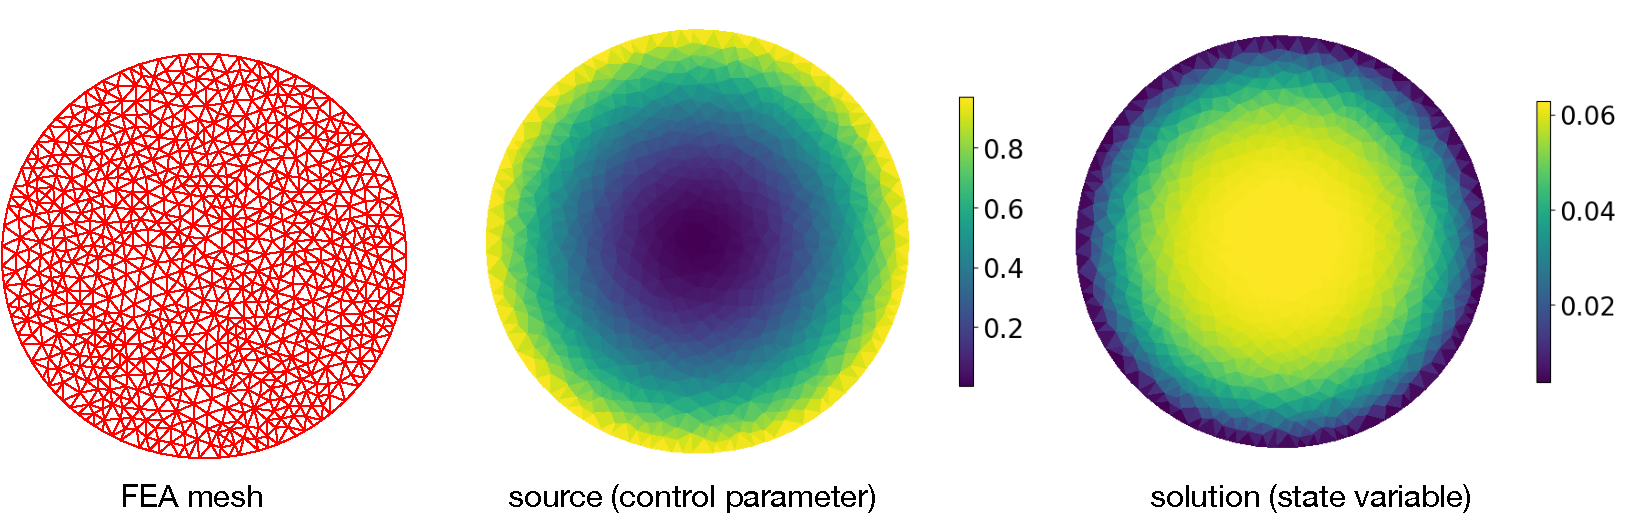
\includegraphics[width=0.8\linewidth]{figures/poisson_equation.pdf}
\caption{Poisson equation on a disc.
Figure: \citet{xue2020amortized}.}%
\label{fig:metapde-poisson}%
\end{figure} \\
When the unknown function $u$ is time dependent (i.e., $du/dt \neq 0$), the PDE problem becomes a Initial Value Problem. One can easily adapt FEM to solve Initial Value Problem by first discretizing the time derivative using a finite difference approximation. At each time step, a Boundary Value Problem is solved independently, and the full solution to the PDE consists of a sequence of time-independent solutions at each time discretization step.\\
We use simple backward finite difference method to approximate the time derivative:
\begin{align}
    \left( \frac{\partial u}{\partial t}\right)^{n+1} \approx \frac{u^{n+1} - u^{n}}{\Delta t} \quad n \in \left \lbrace 0, 1,2,3...N\right\rbrace
\end{align}
The time horizon $[0, T]$ is discretized into a grid of size $N$, with step size $\Delta t = \frac{T}{N}$. Inserting the time discretization into the \emph{strong form} yields:
\begin{align}
    \frac{u^{n+1} - u^{n}}{\Delta t} + \mathcal{N}\left[ u ^{n+1}(\bm{x})\right] &= 0 &\bm{x} \in \Omega, n \in \left \lbrace 0,1,2,3...N\right\rbrace ,  \\
    u^{n+1}(\bm{x}) &= \bar{u} & \bm{x} \in \partial\Omega, n \in \left \lbrace 0,1,2,3...N\right\rbrace , \\
    u^n &= \bar{u}_0(\bm{x}) &\bm{x} \in \Omega, n = 0.
\end{align}
The time discretization step breaks the Initial Value Problem into a sequence of $N$ Boundary Value Problems. At each time step $n$, we solve for $u^{n+1}$ while assuming $u^{n}$ is known from the previous time step. The accuracy of the numerical solution depends on the coarseness of the time grid. 

\subsection{Physics-Informed Neural Networks (PiNN)}
The goal of a PiNN is to its parameters such that it can approximate the solution to the PDE given. In the original proposal, PiNNs can not only incorporate the standard "supervised" data loss, but also a physics-informed loss. The standard supervised loss requires knowing the ground truth solution evaluated at sample points. This "supervised" data loss is useful when experimental data is available. The physics-informed loss consists of the residual of the differential equation. We expect $f_{\theta}$ to satisfy the equations specified above as perfectly as possible. Therefore, one way to incorporate the is to minimize the residual when using $f_\theta$ as the ansatz to the PDE solution $u$. 
\begin{align*}
  \mathcal{J}(u) &= \int_{\Omega} ||\mathcal{N}(u)(\bm{x}, t)||^2_2 dx + \int_{\partial\Omega} ||\mathcal{G}(u)(\bm{x}, t)||_2^2 dx
\end{align*}
During training, we randomly sample collocation points from the PDE domain $\Omega$ and use a set of collocation points $\mathcal{C}$ to approximate the differential equation residual:
\begin{align}
    \mathcal{L}_{\text{PiNN}} = \frac{1}{|\mathcal{C}|} \sum_{(\bm{x}, t) \in \mathcal{C}} || \mathcal{N} (f_{\theta})(\bm{x}, t) ||_2^2  + \frac{1}{|\mathcal{C}|}  \sum_{{(\bm{x}, t) \in \mathcal{\partial \mathcal{C}}} } ||\mathcal{G}(f_{\theta})(\bm{x}, t)||_2^2 
\end{align}
As with \citet{xue2020amortized}, we use this optimization perspective
to derive an efficient training method for our surrogate models.\textcolor{red}{need to complete...}
%\begin{comment}
\section{Surrogate modeling}
Meta-PDE is a surrogate modeling approach.
Surrogate models are useful when one will need to evaluate the solution of many
PDEs from a similar family and is willing to pay the up-front cost of training a
surrogate in order to solve the downstream probelms with minimal cost-per-PDE.
The most popular application is in design or system identification, where a PDE
must be solved at each step optimizing the PDE's parameters, boundary conditions, or geometry,
and it is convenient to replace the PDE solver with a cheap surrogate~\citet{kochenderfer2019algorithms}.
The optimization may be numerical ("PDE-constrained optimization") or by hand.
If numerical, gradients can be obtained using the adjoint method with cost equivalent
to one solve of a linearized version of the PDE.
In both cases, therefore, the optimization bottleneck is in the "forward pass" of solving the PDE.
Surrogate models are also particularly relevant in scenarios involving dynamics models
(where a PDE must be solved at each timestep),
and where real-time analysis is required for the convenience of a human designer or
to allow embedding the PDE solver in a control policy.

There are many approaches to surrogate modeling, such as
random forests~\citep{criminisi2011decision},
Gaussian processes~\citep{shahriari2015taking},
Student-$t$ processes~\citep{shah2014student},
and neural networks~\citep{snoek2015scalable}.
Regression can be from the PDE's parameters to coefficients of the PDE solution,
yielding a general-purpose surrogate for that distribution of PDEs, or from
PDE parameters to an objective value for a specific optimization problem.
Most surrogate modeling procedures have two key restrictions:
\begin{enumerate}
  \item They require supervised training data in the form of
  (PDE parameter, PDE solution) or (PDE parameter, objective value) pairs,
  which must be generated by an expensive ground-truth PDE solver, \label{itm:supervision}
  \item They regress from a vector representation of the PDE or its parameters to a
  vector representaion of the solution; having to fix these vector bases
  makes it difficult to fit surrogates for
  distributions of PDEs containin highly varied structure in geometry or governing
  equations.\label{itm:structure}
\end{enumerate}
Restriction \ref{itm:supervision} means that in order to be of net computational benefit,
the surrogate must be applied to many more downstream problems than the number of
data points required to fit a good model. For rich classes of PDEs and expressive models,
it can take tens or hundreds of thousands of data points to fit a model which can generalize,
so this greatly limits surrogate models' use case.

Restriction \ref{itm:structure} is not an issue if the problem can be phrased as
regressing from coefficients of a parameter or boundary condition in a piecewise polynomial
basis to coefficients of a solution in a similar basis, with the discretization
fixed across problems.
However, many problems are not amenable to such framing.
Problems with different domain geometry or very different parameters and solutions
may require very different discretizations to represent them well;
generating a good mesh for a given problem can itself be a hard problem and can be a
greater bottleneck than the cost of the base PDE solve.
The factors of variation of a PDE (the domain, governing equations, and parameters)
are naturally and generally expressed as functions on the domain and as
operators on solutions: requiring them to be parameterized by vectors restricts
the classes of PDEs to which surrogate models can be applied and greatly limits their
use case.

Several recent works have relaxed one of these restrictions.
\citet{zhu2019physics} amortize the finite differentce method,
predicting PDE solutions from parameter fields with a
ConvNet by training the ConvNet to produce solutions with minimum variational energy
across a distribution of problems.
This removes restriction \ref{itm:supervision} but requiring the discretization
to be a fixed uniform grid.
\citet{xue2020amortized} amortize the finite element method, training a surrogate model
to minimize a similar variational energy but use a finite element discretization:
their model can handle complicated geometry, and by measuring the variational energy
in the finite element basis maintains some desirable properties of finite element
analysis. This avoids restriction \ref{itm:supervision} and allows arbitrary
meshes but requires a single mesh be fixed for all PDEs in the distribution to be
amortized.
Graph Neural Network based approaches \citep{sanchez2020learning,pfaff2020learning},
which learn a forward operator in terms of
interactions between nearby particles or mesh cells,
allow for arbitrary geometries (partially removing restriction
\ref{itm:structure})
but require supervised data and have not yet produced surrogate models which are
cheaper to evaluate than ground-truth solvers when tested on equivalent hardware.
Neural Operator based approaches \citep{li2020neural,li2020fourier} learn a map from
initial conditions or parameters to solution which builds in
some invariance to mesh \emph{resolution}, but require the mesh to be a uniform
grid, and also require expensive supervised data.
\end{comment}
%% \section{Solving PDEs with neural networks}
% \begin{itemize}
%  \item NN bases: mesh-free; instead of needing to generate a mesh,
%  need to provide a sampler and loss function. Sometimes easier
%  than generating a good discretization.
 % \item Physics-informed NNs: given known governing equations
% and some supervised data, fit a NN solution which incorporates both.
% More flexible than PDE-CO on boundary conditions to fit the data.
% \item But solving PDEs with NNs is super slow.
% \end{itemize}

\section{Meta-learning mesh-free PDE operators}
We consider time-dependent PDEs
\begin{align}
\frac{\partial}{\partial t}u(\bm{x}, t) + \mathcal{N}\left[ u(\bm{x}, t)\right] &= 0 &\bm{x} \in \Omega, t \in [0, T], \label{eq:metapde-time-strongform} \\
G(u)(\bm{x}, t) &= 0 & \bm{x} \in \partial\Omega, t \in [0, T], \label{eq:metapde-time-bc} \\
u(\bm{x}, 0) &= \bar{u}_0(\bm{x}) &\bm{x} \in \Omega, t=0, \label{eq:metapde-time-ic} 
\end{align}
as well as time-independent PDEs which only have spatial dependence:
\begin{align}
\mathcal{N}\left[ u(\bm{x})\right] &= 0 & \bm{x} \in \Omega, \label{eq:metapde-space-strongform} \\
G(u)(\bm{x}) &= 0 & \bm{x} \in \partial\Omega. \label{eq:metapde-space-bc}
\end{align}
The problem is defined on the spatial domain $\Omega \subset \mathbb{R}^{d}$ with boundary $\partial \Omega$. For time-dependent PDEs the time horizon is $[0, T]$. 
%The unknown function in the PDE $u(\bm{x}, t)$ is a function of the spatial coordinate $\bm{x}$ and time coordinate $t$. 
%$\partial / \partial t u(\bm{x}, t) $ is the partial derivative of the unknown function $u$ with respect to the time. 
%$\mathcal{N}\left[ u(\bm{x}, t)\right]: (\Omega \to \mathbb{R}^{d_u}) \to (\Omega \to \mathbb{R}^{d_\mathcal{F}})$ is an operator that involves $u$ and the partial derivatives of $u$ with respect to its spatial coordinates $\bm{x}$.
In both cases $\mathcal{N}$ is an operator that involves $u$ and the partial derivatives of $u$ with respect to its spatial coordinates $\bm{x}$.

%Figure \ref{fig:metapde-poisson} shows as an example the Poisson problem on a disc. For this simple problem we have $\mathcal{F}(u) = \nabla^2 u - f$, for a spatially varying source term $f$, and $\mathcal{G}(u) = u$, i.e. enforcing $u=0$ on the boundary. 
%\begin{figure}[t]
%  \centering
%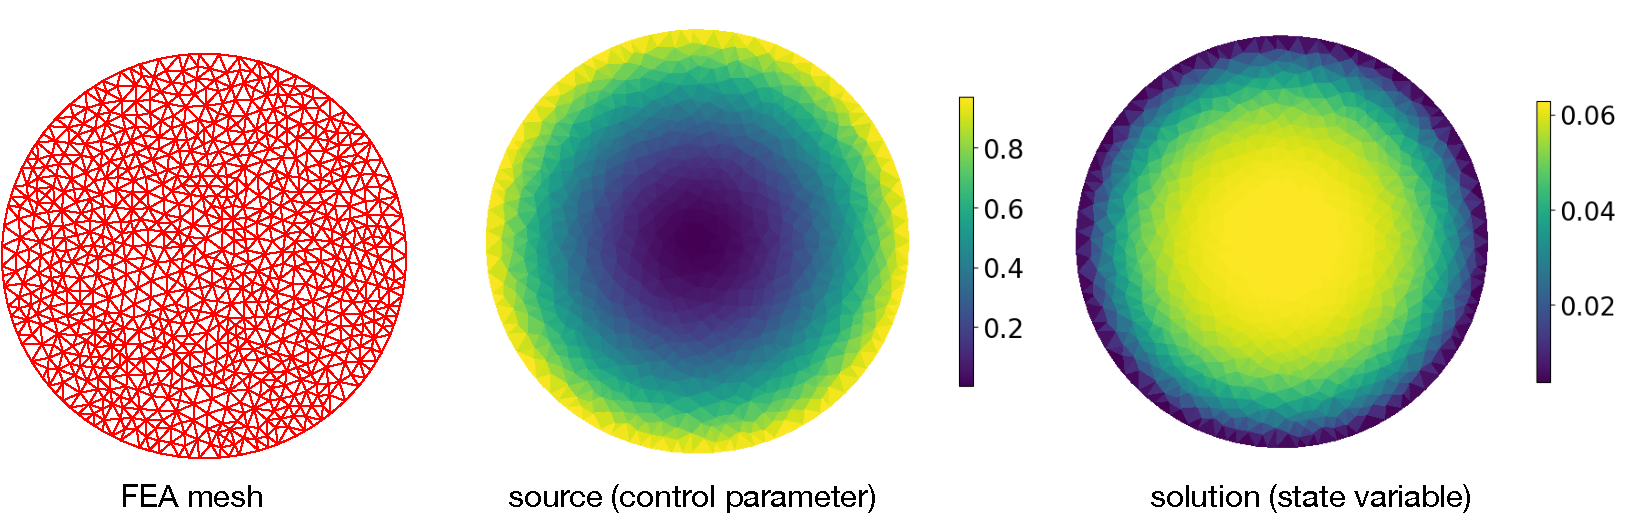
\includegraphics[width=0.8\linewidth]{figures/poisson_equation.pdf}
%\caption{Poisson equation on a disc.
%Figure: \citet{xue2020amortized}.}%
%\label{fig:metapde-poisson}%
%\end{figure} \\
\subsection{Physics-Informed Neural Networks (PINN)}
The goal of a PINN is to represent the solution ansatz $u(\bm{x},t)$ with a neural network $f_\theta(\bm{x},t)$. 
Doing so requires learning $\theta$ such that $f_\theta$ approximates the solution to the PDE over the problem domain.
Learning these parameters is an optimization problem, which requires defining a loss function whose minimum is the solution of the PDE.
%In the original proposal, PINNs can not only incorporate the standard "supervised" data loss, but also a physics-informed loss. 
%The standard supervised loss requires knowing the ground truth solution evaluated at sample points. 
%This "supervised" data loss is useful when experimental data is available. 
%The physics-informed loss consists of the residual of the differential equation. 
%Therefore, one way to incorporate the is to minimize the residual when using $f_\theta$ as the ansatz to the PDE solution $u$. 
We choose a `physics-informed loss' which consists of the residual of the differential equation over the problem domain and boundary. For time-independent PDEs, this loss function is
\begin{align}\label{eq:pinn_loss_function}
  \mathcal{J}(u) &= \int_{\Omega} \left|\left| \mathcal{N}(u)(\bm{x})\right|\right|^2_2 \, dx + \int_{\partial\Omega} \left|\left| \mathcal{G}(u)(\bm{x})\right|\right| _2^2 \, dx.
\end{align}
For time-dependent PDEs, this loss function is: 
\begin{align}\label{eq:pinn_loss_function}
  \mathcal{J}(u) = & \int_{\Omega} \left|\left| \frac{\partial}{\partial t}u(\bm{x}, t) + \mathcal{N}(u)(\bm{x}, t)\right|\right|^2_2 \, dx + \\
  & \int_{\partial\Omega} \left|\left| \mathcal{G}(u)(\bm{x}, t)\right|\right| _2^2 \, dx + \int_{\Omega} \left|\left| u(\bm{x}, 0) - \bar{u}_0(\bm{x}) \right|\right| _2^2 \, dx .
\end{align}
During training, we randomly sample collocation points from the PDE domain $\Omega$ and boundary $\partial \Omega$ and use these points $\mathcal{C} \in \Omega$ and $\partial \mathcal{C} \in \partial \Omega$ to approximate the differential equation residual. For time-independent PDEs, the training loss is
\begin{align}\label{eq:pinn_training_loss}
    \mathcal{L}_{\text{PINN}}(f_\theta) = \frac{1}{|\mathcal{C}|} \sum_{\bm{x} \in \mathcal{C}} \left|\left| \mathcal{N} (f_{\theta})(\bm{x}) \right|\right|_2^2  + \frac{1}{|\partial \mathcal{C}|}  \sum_{{\bm{x} \in \mathcal{\partial \mathcal{C}}} } \left|\left|\mathcal{G}(f_{\theta})(\bm{x})\right|\right|_2^2.
\end{align}
For time-dependent PDEs, the training loss is
\begin{align}\label{eq:pinn_training_loss}
    \mathcal{L}_{\text{PINN}}(f_\theta) = & \frac{1}{|\mathcal{C}|} \sum_{\bm{x} \in \mathcal{C}}\left|\left| \frac{\partial}{\partial t}(f_\theta)(\bm{x}, t) + \mathcal{N} (f_{\theta})(\bm{x}, t) \right|\right|_2^2  +\\ 
     & \frac{1}{|\partial \mathcal{C}|}  \sum_{{\bm{x} \in \mathcal{\partial \mathcal{C}}} } \left|\left|\mathcal{G}(f_{\theta})(\bm{x}, t)\right|\right|_2^2 + \frac{1}{|\mathcal{C}|} \sum_{\bm{x} \in \mathcal{C}} \left|\left| f_{\theta}(\bm{x}, 0) - \bar{u}_0(\bm{x}) \right|\right| _2^2.
\end{align}

When the training converges, we expect $f_{\theta}$ to approximately satisfy the above equations, meaning that $\mathcal{L}_{\text{PINN}}(f_\theta)$ should be nearly zero.
%As with \citet{xue2020amortized}, we use this optimization perspective to derive an efficient training method for our surrogate models.

\subsection{Meta-PDE Method}

This lets us develop a new, ``functional'' API for surrogate modeling.
%, which can handle arbitrary geometries and removes the need to fix a mesh or to fix vector bases for the PDE parameters or solution.
For a given PDE, our surrogate model takes as input: 
\begin{itemize}
    \item[(i)] Samplers which can sample points uniformly on each region of the domain.
    \item[(ii)] A loss function encoding the PDE constraint or boundary condition for each such region.
\end{itemize}
Combining these allows estimation of the residual which measures deviation of a given solution field from the governing equations. We use a neural network to model the solution field, and train a neural network initialization to converge quickly across a distribution of tasks; in our case each task in the distribution is minimizing the residual for a PDE or minimizing the variational energy for the PDE with given domain, boundary conditions and governing equations. 

In this work, we use gradient-based meta-learning to amortize the training time needed to fit each parametrization of the PDE. The LEAP-based Meta-PDE method learns the model initialization $\theta^0$ for a neural network $f_\theta$. $f_\theta$ can be trained to approximate the solution $u: \mathbb{R}^{d_\Omega} \to \mathbb{R}^{d_u}$ of an individual parametrization of the PDE. To learn $\theta^0$, we start with a distribution of tasks, with each task specified by samplers and constraint operators for the boundary and loss. Each task in this distribution represents a different parametrization of the PDE. Then we draw a batch of $n$ tasks with individual loss functions $\hat{\mathcal{L}}_i$, $i \in [n]$. The initialization for each inner task is $\theta^0$, and is updated by the inner gradient update rule. During each inner gradient update, we update the meta-gradient per LEAP algorithm. We unroll the inner learning loop $K$ steps to find $f_{\theta_i^K}$: the solution ansatz for each task $i$ in the batch. After unrolling $K$ update steps for $n$ tasks, we update the learned model initialization $\theta^0$ with the meta-gradient:
\begin{align}
    \theta^0 \leftarrow \theta^0 - \beta \nabla_{\theta^0}\sum_{i=1}^n \frac{1}{n} d(\theta^0; M_i),
\end{align}
where $d(\theta^0; M_i)$ is the distance of the gradient path for task $i$ on its manifold $M_i$, as specified in \citep{flennerhag2018transferring}.

The MAML-based Meta-PDE method learns the model initialization $\theta^0$ for a neural network $f_\theta$ and also learns the inner gradient update rule. We use SGD as the inner gradient update rule and MAML learns the optimal step size for each parameter in $\theta$ for each inner each step. For each task the loss is $\hat{\mathcal{L}}_i(f_{\theta_K, i})$. We perform backpropagation through the inner loop to find the gradients w.r.t meta-initialization $\theta_0$ and use the gradients to update $\theta_0$ in the outer loop training:
\begin{align}
    \theta^0 \leftarrow \theta^0 - \beta \nabla_{\theta^0} \sum_{i=1}^n  \frac{1}{n} \hat{\mathcal{L}}_i(f_{\theta^K _i})
\end{align}
We also perform backpropagation through the inner loop to find the gradients w.r.t. the per-step, per-parameter step size $\alpha$ and use the gradients to update the $\alpha$ in the outer loop training:
\begin{align}
    {\alpha}  \leftarrow {\alpha} - \beta  \nabla_{\alpha} \sum_{i=1}^n  \frac{1}{n} \hat{\mathcal{L}}_i(f_{\theta^K_i})
\end{align}

The Meta-PDE surrogate model is designed to have an input schema as close to this general specification as possible. Most PDEs can be fully defined by specification of:
\begin{itemize}
  \item a domain $\Omega$ with boundary $\partial \Omega$,
  \item an operator $\mathcal{F}$ representing governing equations,
  \item and an operator $\mathcal{G}$ representing boundary conditions.
\end{itemize}
When using Meta-PDE as a surrogate to compute an approximate solution to a given paramterization of the PDE (one task), the inputs to the Meta-PDE model immitate the general. specification above:
\begin{itemize}
  \item a sampler $s(\Omega)$ which returns points in the domain $\Omega$,
  \item a sampler $s(\partial\Omega)$ which returns points on the boundary $\partial\Omega$,
  \item an operator $\mathcal{F}$ representing governing equations,
  \item and an operator $\mathcal{G}$ representing boundary conditions.
\end{itemize}
The operators $\mathcal{F}$ and $\mathcal{G}$ may be supplied directly and do not require a particular parametric form. The geometric dimension $\mathbb{R}^{d_\Omega}$ and solution dimension $\mathbb{R}^{d_u}$ must remain fixed across PDEs in the distribution, even though $\Omega$ is allowed to vary. The samplers and operators are sufficient to construct an estimator $\hat{\mathcal{L}}$ for the task loss $\mathcal{L}$:
\begin{align}
  \mathcal{L}(u) &= \int_{\Omega} \big|\big|\mathcal{F}(u)(\bm{x})\big|\big|^2_2 d\bm{x} +
  \int_{\partial\Omega} \big|\big|\mathcal{G}(u)(x)\big|\big|_2^2 d\bm{x} \\
  \hat{\mathcal{L}}(u) &= \mathbb{E}_{x \sim s(\Omega)} \big|\big|\mathcal{F}(u)(\bm{x})\big|\big|^2_2 +
  \mathbb{E}_{\bm{x} \sim s(\partial \Omega)} \big|\big|\mathcal{G}(u)(\bm{x})\big|\big|_2^2
\end{align}
$\hat{\mathcal{L}}(f)$ is unbiased as long as $s(\cdot)$ return points with uniform probability over their supports, or return batches of points which have uniform probability for any given $x$ aggregated over the batch. Unbiased estimation is not necessarily essential. Note $\hat{\mathcal{L}}(f) > 0$ and $\mathcal{L}(f) > 0$ $\forall f$, and the true solution $u$ of the PDE achieves $\mathcal{L}(u) = \hat{\mathcal{L}}(u) = 0$. These properties hold if we multiply the integrand in $\mathcal{L}(f)$ by an arbitrary density $\mu > 0$ or if we choose samplers $s$ which have full support but nonuniform probability on $\Omega$ or $\partial \Omega$. Therefore, biased sampling will not change the minimizer of the energy estimator if we have a sufficiently expressive hypothesis class for $f$.

%The user must supply a sampler for the domain and for the boundary of each PDE within the training distribution and for each PDE seen during deployment. A sampler can easily be constructed for any domain for which we have a mesh, but it is also often easier to construct a sampler than to construct an accurate mesh.
During deployment time, a "forward pass" computes an approximate solution for a given PDE parametrization with $K$ steps of stochastic optimization steps. The $K$ gradient steps minimize the residual for the task $\mathcal{L}(f)$. If the model has been trained with LEAP-based Meta-PDE method, it will start from the meta-learned model initialization $\theta_0$. If the model has been trained with MAML-based Meta-PDE method, it will start from the meta-learned model initialization $\theta_0$ and the step size $\alpha$ will be also be specified for each parameter and each step: 
\begin{align}
  \theta^k = \theta^{k-1} - \alpha \nabla_{\theta^{k-1}} \hat{\mathcal{L}}(f_{\theta^{k-1}}) \quad k = 1 .. K
\end{align}
In both cases, the Meta-PDE method returns the approximate solution $f_{\theta^K}$, the neural network with the final set of parameters. One could further fine tune the model beyond $K$ gradient steps to achieve higher solution accuracy at the cost of longer solving time. 

Finite element analysis methods usually use piecewise linear meshes, which can take many elements to accurately represent curved shapes: even when using piecewise polynomially-shaped meshes, the slow rate of convergence of using these meshes to approximate non-polynomial geometry can be a major source of error and/or computational expense for FEA. In the next section, we will further explore the accuracy/time trade-off for Meta-PDE during deployment, and compare it with the accuracy/time trade-off for FEA methods. 

%Given an inside-outside oracle for the domain, it is easy to use rejection sampling to sample from it exactly. Most parametric geometry representations such as those used in computer-aided design also allow exact sampling of the boundary, and even minimal representations such as signed distance functions allow approximate sampling \citep{brubaker2012family}.

\section{Experiments}
We evaluate the application of Meta-PDE to three example PDE problems: the nonlinear Poisson's Equation, the 1D Burgers’ Equation, and the Hyper-elasticity Equation. We compare Meta-PDE's performance with baseline solved by the numerical solver Fenics.
\subsection{Nonlinear Poisson Equation}
Poisson's Equation is one of the most ubiquitous equations in physics. For example, the linear Poisson's Equation calculates electrostatic or gravitational field causes by electric charges or mass particles. Since the linear Poisson's Equation can be solved analytically, we demonstrate Meta-PDE on a nonlinear Poisson problem with varying source terms, boundary conditions, and geometric domain. The nonlinear Poisson's Equation takes the form:
\begin{align*}
\nabla \cdot \left[ (1 + 0.1 u^2) \nabla u(\bm{x}) \right]&= f(\bm{x}) \quad &\bm{x} \in \Omega\\
u(\bm{x}) &= b(\bm{x}) \quad &\bm{x} \in \partial\Omega
\end{align*}
where $u \in \mathbb{R}^1$ and $\Omega \subset \mathbb{R}^2$. Using our notation from the previous section, this is equivalent to constraining the solution in the domain with an operator~${\mathcal{F}(u) = ((1 + 0.1 u^2) \nabla u) - f}$, and constraining the solution on the boundary with an operator~${\mathcal{G}(u) = u - b}$.

The domain $\Omega$ is a disc-like shape centered at the origin, defined in polar coordinates by  and the varying radius about the origin
\[
r(\theta) = r_0[1 + c_1 \cos(4\theta) + c_2 \cos(8\theta)],
\]
where the varying parameters are $c_1, c_2 \sim \mathcal{U}(-0.2, 0.2)$. The source term $f$ is a sum of radial basis functions,
\[
f(\bm{x}) = \sum_{i=1}^3 \beta_i \exp{||\bm{x} - \mu_i||_2^2},
\]
where $\beta_i \in \mathbb{R}^1$ and $\mu_i \in \mathbb{R}^2$ are both drawn from standard normal distributions. The boundary condition $b$ is a periodic function, defined in polar coordinates as
\[
b(x) = b_0 + b_1 \cos(\theta) + b_2 \sin(\theta) + b_3 \cos(\theta) + b_4 \sin(\theta),
\]
where the parameters $b_{0:4} \sim \mathcal{U}(-1, 1)$.
%Figure \todo{make fig} shows the domain, source term, and boundary conditions across several sampled PDEs.

Our MAML-based Meta-PDE model is a small NN (3 layer with layer size 64) with sinusoidal activation functions. The sinusoidal activation is initialized according to the scheme in \citet{sitzmann2020implicit}, although we replace $\omega_0 = 30.0$ in that paper with $\omega_0 = 3.0$ to avoid numerical issues when taking higher-order derivatives of a neural network's input-output function. The inner-loop (task-specific learning) takes 5 gradients steps to adapt the NN solution to a different PDE problem. We initialize the inner-loop learning rate to $1\times 10^{-4}$, and use an outer loop learning rate of $1\times 10^{-5}$. Gradients in both inner and outer loop are clipped to have maximal norm $100.0$. In the inner loop, we use vanilla SGD. In the outer loop, we use the Adam optimizer \citep{kingma2014adam}. 

Our LEAP-based Meta-PDE model uses the same architecture (3 layer with layer size 64) and sinusoidal activations between layers. The inner-loop (task-specific learning) takes 60 gradients steps. We initialize the inner-loop learning rate to $2.5\times 10^{-5}$, and use an outer loop learning rate of $5\times 10^{-5}$. Different from our MAML-based Meta-PDE model, we use  Adam optimizer \citep{kingma2014adam} for both inner loop optimizations (task-specific optimization) and the outer loop optimization (meta-learning).

\begin{wrapfigure}[20]{r}{0.6\textwidth}
  \centering
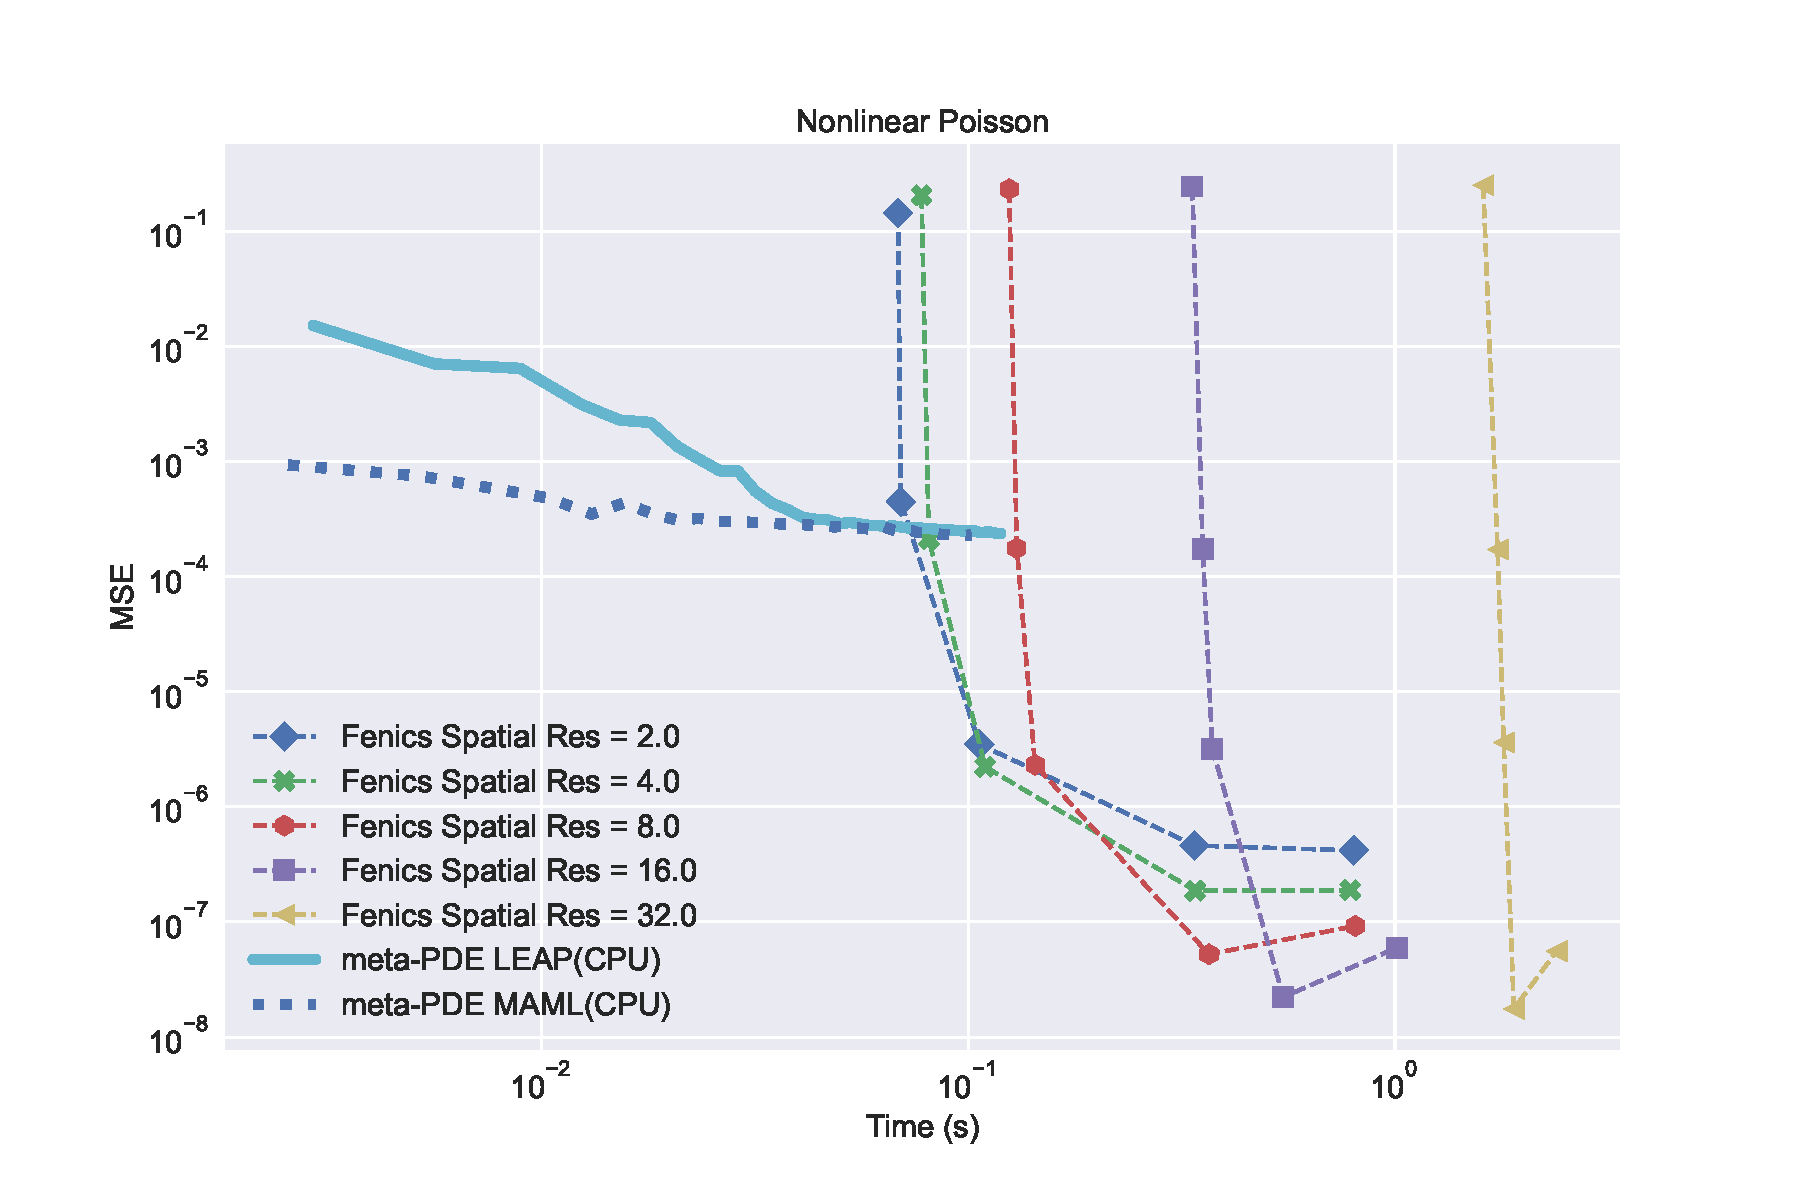
\includegraphics[width=\linewidth]{figures/poisson.pdf}
\caption{MSE of each solution and the solving time required for the desired accuracy.}%
\label{fig:poisson_summary}%
\end{wrapfigure}

We train both Meta-PDE methods with a batch size of 16 tasks. For each task, we sample 1024 sampled points on the boundary and 1024 points in the domain to evaluate the residual at each inner optimization step. 
We sample points uniformly on the domain and the boundary, which gives us strong performance. If needed, we could also divide the domain into subdomains which could lead to further variance reduction.
%To sample points on the boundary, we construct an evenly spaced interval mesh of angles in $[0, 2\pi]$, add uniform noise of the size of one interval to each point, and use the points on the boundary using these angles. To sample points in the domain, we do the same but also draw random radii uniformly in $[0, r(\theta)]$. These samplers are not unbiased for non-circular shapes, but this does not change the optimal solution. 
Meta-PDE methods are implemented in Jax \citep{jax2018github}. For the MAML-based Meta-PDE method, we train for 120,000 outer-loop steps, which takes about 4 hours on one NVIDIA T4 GPUs. For the LEAP-based Meta-PDE method, We train for 55,000 outer-loop steps, which takes about 5 hours on NVIDIA T4 GPUs. All finite element baselines are implemented in FEniCS \citep{LoggMardalEtAl2012a,AlnaesBlechta2015a}. We use the Mumps linear solver backend. Figure \ref{fig:results_per_step} shows the ground truth (baseline) solution for eight PDE problems used in the validation set. The same figure also shows the MAML meta-learned initialization, which can quickly adapt to each PDE problems in five gradient steps. 
\begin{SCfigure}[1.0][t]
 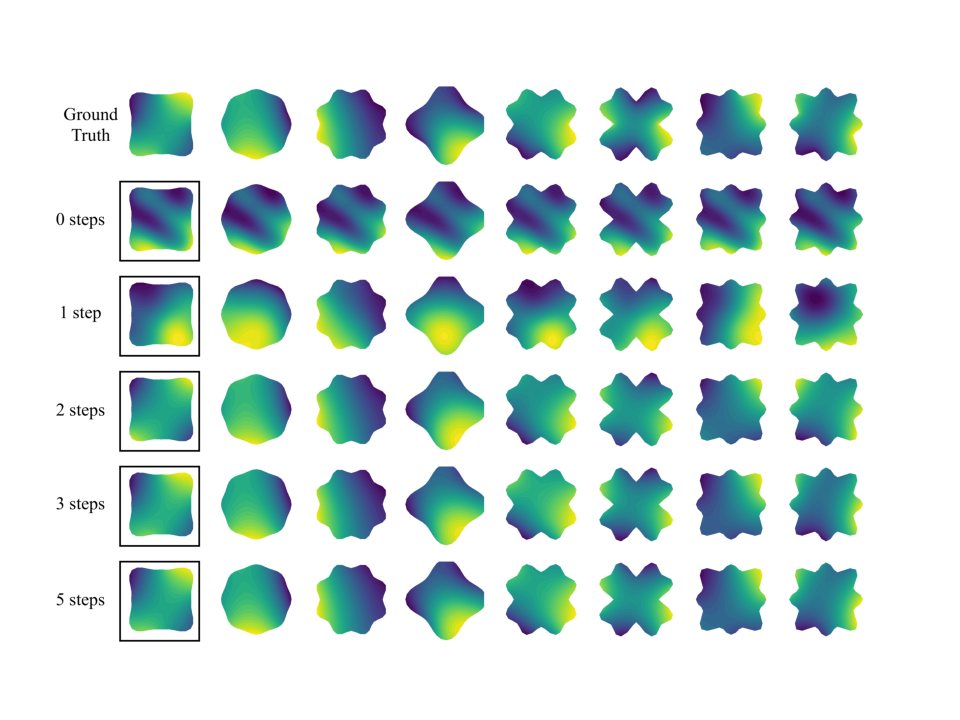
\includegraphics[width=1.4\linewidth]{figures/poisson_meta.pdf}
\caption{Solutions to nonlinear Poisson's equations with varying domains, boundary conditions and source terms. Top: ground truth finite element solution. Second row: solution represented by Meta-PDE initial neural network parameters. Third row onwards: solution after each gradient step in the Meta-PDE inner loop.}
\label{fig:results_per_step}
\end{SCfigure}

% FENICS
% res: 1, rel_mse: 0.28237417340278625, std_rel_mse: 0.6290896534919739, time: 0.05341055989265442
% res: 2, rel_mse: 0.014543757773935795, std_rel_mse: 0.029957808554172516, time: 0.12654799222946167
% res: 3, rel_mse: 0.006523779593408108, std_rel_mse: 0.013875527307391167, time: 0.23686206340789795
% res: 4, rel_mse: 0.0011952054919674993, std_rel_mse: 0.0021807190496474504, time: 0.4497535675764084
% res: 5, rel_mse: 0.0007102875970304012, std_rel_mse: 0.0014738228637725115, time: 0.7402735650539398
% res: 6, rel_mse: 0.0003710805904120207, std_rel_mse: 0.0008687296649441123, time: 0.8322657346725464
% res: 8, rel_mse: 4.029081901535392\times 10^{-05, std_rel_mse: 5.9528952988330275\times 10^{-05, time: 1.23470838367939
% res: 10, rel_mse: 2.8872436814708635\times 10^{-05, std_rel_mse: 6.197320180945098\times 10^{-05, time: 1.8577006310224533
% res: 12, rel_mse: 5.06512105857837\times 10^{-06, std_rel_mse: 9.67413689068053\times 10^{-06, time: 2.4609854966402054

% Us
% maml_poisson_outer1en5_inner1en4_outerclip1e2_innerclip1e2
% time: 0.0022 // 0.19 s
% err: 0.00013, std 0.00027

% \begin{table}
%\begin{adjustbox}{max width=\textwidth}
%\begin{tabular}{|c|ccccc|}
% \hline
% Method & Resolution & Mean finite element DoFs & Relative MSE & Simulation time (CPU) % & Simulation time (GPU) \\
% \hline
% FEA & 1 & 15 & $0.28 \pm 0.63$ & 0.053s & N/A \\
% FEA & 2 & 53 & $0.014 \pm 0.030$ & 0.13s & N/A \\
% FEA & 3 & 85 & $0.0065 \pm 0.014$ & 0.24s & N/A \\
% FEA & 4 & 178 & $0.0012 \pm 0.0022$ & 0.45s & N/A \\
% FEA & 5 & 222 & $7.1\times 10^{-4} \pm 1.5\times 10^{-3}$ & 0.74s & N/A \\
% FEA & 6 & 324 & $3.7\times 10^{-4} \pm 8.7\times 10^{-4}$ & 0.83s & N/A \\
% FEA & 8 & 433 & $4.0\times 10^{-5} \pm 6.0\times 10^{-5}$ & 1.2s & N/A \\
% FEA & 10 & 568 & $2.9\times 10^{-5} \pm 6.2\times 10^{-5}$ & 1.9s & N/A \\
% FEA & 12 & 1246 & $5.1\times 10^{-6} \pm 9.7\times 10^{-6}$ & 2.5s & N/A \\
% FEA & 16 & 2163  & $5.1\times 10^{-6} \pm 9.7\times 10^{-6}$ & 2.92s & N/A \\
% Meta-PDE & N/A & N/A & $6.2\times 10^{-5} \pm 1.0\times 10^{-4}$  & 0.097s & 0.0022s % \\
% \hline
% \end{tabular}
% \end{adjustbox}
% \caption{
% Accuracy vs solution time for finite element methods and for meta-PDE. For FEA, a mesh % is generated with MSHR using 3x "resolution" points to define the geometry, and % "resolution" as an argument to MSHR's automeshing too.}
% \label{tbl:results}
% \end{table}
During deployment, the Meta-PDE solutions could be further improved by extending the number of "inner" training steps beyond what is specified in the Meta-PDE method. In our MAML-based Meta-PDE method for example, we first initialize the NN with the meta-learned initialization. We then perform the 5 inner-gradient steps training. After the 5 inner-gradient steps, we have the optionality to continue fitting the NN for a particular instance of PDE. The goal of further training is to fine-tune the NN to better fit a particular instance of the PDE problem. We compare the speed/accuracy trade-off of our Meta-PDE method during deployment time with the FEA method. Figure \ref{fig:poisson_summary} shows the mean squared error (MSE) of each solution and solving time required for the desired accuracy. The highest-fidelity FEA method was taken as ground truth and was used to compute MSE. The MSE and solving times were evaluated using 8 held-out problems from the same distribution, and the 8 held-out problems were not used during training. Mean-squared errors are computed between the value of a given approximate solution and the value of the ground truth (highest fidelity finite element solution) at 1024 randomly sampled points within the domain. The held-out set configuration remains the same for the other two experiements below. 

% The relative mean-squared error is computed by dividing the mean-squared error by the sum of squares of solution values for the ground-truth solution.
%Figure \todo{make} shows the ground truth and finite element approximations of various fidelities for sampled test problems. 
%Figure \ref{fig:results_per_step} shows the ground truth and the Meta-PDE solution after zero through five gradient steps minimizing the variational energy for sampled test problems.\\

We see that Meta-PDE learns to output accurate solutions, and when run on the same CPU (3.6 GHz Intel Xeon Platinum 8000 series) is about $10\times - 20\times$ faster than a finite element method with similar accuracy.
%and about $?\times$ more accurate than a finite element method with the same computation cost. Unlike finite element models, Meta-PDE can be easily accelerated by a GPU, and on GPU we see close to $?\times$ speed up in deployment, leading to a $?\times$ speed increase over similar accuracy finite element models.






\subsection{Burger's Equation}
The Burger's Equation is a time-dependent PDE that models the system consisting of a moving viscous fluid. The 1D version of the equation models the fluid flow through an ideal thin pipe. The strong form of Burger's Equation is given by:
\begin{align}
    \frac{\partial u}{\partial t} + u \frac{\partial u}{\partial x} - \nu \frac{\partial ^2 u}{\partial x^2} &= 0, \quad & x \in \Omega, t \in [0, T] \\
    u(x, 0) &= u_0(x), \quad & x \in \Omega \\
    u(x, t) &= \bar{u}, \quad & x \in \partial \Omega, \in (0, T] 
\end{align}
Variable $x$ represents the spatial coordinate, and is defined on the spatial domain $\Omega$. Variable $t$ represents the temporal coordinate and the corresponding domain lives in $[0, T]$. Function $u_0(x)$ is the initial condition for the PDE and $\bar{x}$ is the boundary condition. The unknown $u(x, t)$ is the speed of the fluid, which is a function of position $x$ and time $t$. $\nu$ is the viscosity of the fluid. If the viscosity $\nu$ of the fluid is low, the fluid develops a shock wave, which is a characteristic of viscous Burger's Equation.
\begin{table}[htbp]
\caption{Neural Network hyperparameter sets for our Meta-PDE methods}
\label{tbl:hparams}
\centering
\begin{adjustbox}{max width=\textwidth}
\begin{tabular}{llllllll}
    \toprule
    PDE Problem & Meta-PDE Method & \multicolumn{6}{c}{Hyperparameters}  \\
    &  & Num. of layers & Layer Size & Activation & Inner Steps & Inner LR & Outer LR \\
    \midrule
    Nonlinear Poisson's & \multirow{3}{*}{MAML} & 3 &  \multirow{3}{*}{64} & \multirow{3}{*}{$\sin$} &  \multirow{3}{*}{5} & $1.0\times10^{-4}$ & $1.0\times10^{-5}$  \\
    Burger's &  & 8 &  &  &  & $1.0\times10^{-4} $ & $1.0\times10^{-5}$ \\
    Hyper-elasticity &  & 5 &  & &  & $5.0\times10^{-6} $ & $5.0\times10^{-6}$  \\
    \bottomrule
    Nonlinear Poisson's & \multirow{3}{*}{LEAP} & 5 & 64 & \multirow{3}{*}{$\sin$} & 60 & $2.5\times10^{-5} $ & $5.0\times10^{-5}$  \\
    Burger's &  & 10 & 128 & & 80 & $1.0\times10^{-6} $ & $5.0\times10^{-5}$  \\
    Hyper-elasticity &  & 10 & 128 &  & 20 & $1.0\times10^{-5} $ & $1.0\times10^{-5}$  \\
    \bottomrule
  \end{tabular}
\end{adjustbox}
\end{table}

\begin{table}[htbp]
\caption{\small 
Training hyperparameter set for our meta-PDE methods and corresponding training time on one NVIDIA T4 GPUs}
\label{tbl:training}
\centering
\begin{adjustbox}{max width=\textwidth}
\begin{tabular}{llllllll}
    \toprule
    PDE Problem & Meta-PDE Method & \multicolumn{6}{c}{Hyperparameters}  \\
    & & Batch Size & Sampled Points & Iterations & Training Time & Inner Optimizer & Outer Optimizer \\
    \midrule
    Nonlinear Poisson's & \multirow{3}{*}{MAML} & \multirow{3}{*}{8} & 2048 & 120,000 & 4 hrs & \multirow{3}{*}{SGD} & \multirow{3}{*}{Adam} \\
    Burger's &   &  & 1024 & 60,000 & 11 hrs  &  & \\
    Hyper-elasticity &   &  & 1024 & 180,000 & 21 hrs &  & \\
    \midrule
    Nonlinear Poisson's & \multirow{3}{*}{LEAP}  & \multirow{3}{*}{8} & 4096 & 55,000 & 5 hrs  &  \multirow{3}{*}{Adam} &  \multirow{3}{*}{Adam}\\
    Burger's &   &  & 2048 & 7,000 & 7 hrs &  & \\
    Hyper-elasticity &   &  & 1024 & 140,000 & 8 hrs &  & \\
    \bottomrule
  \end{tabular}
\end{adjustbox}
\end{table}

The NN hyperparameter set is in Table \ref{tbl:hparams} and training hyperparameter details are in Table \ref{tbl:training}. All finite element baselines are implemented in FEniCS \citep{LoggMardalEtAl2012a,AlnaesBlechta2015a}. Finite different method is applied on the time-dimension with implicit Euler discretization. For the ground truth comparison, the the time domain $[0, T], T = 1.0s$ is divided into time grid of size 200 with grid size $dt = 5.0\times10^{-3}s$. We use the Mumps linear solver backend. Figure \ref{fig:burgers_per_step} shows the ground truth (baseline) solution for eight PDE problems used in the validation set. The same figure also shows the MAML meta-learned initialization, which can quickly adapt to each PDE problems in five gradient steps. 

\begin{SCfigure}[0.8][htbp]
  \centering
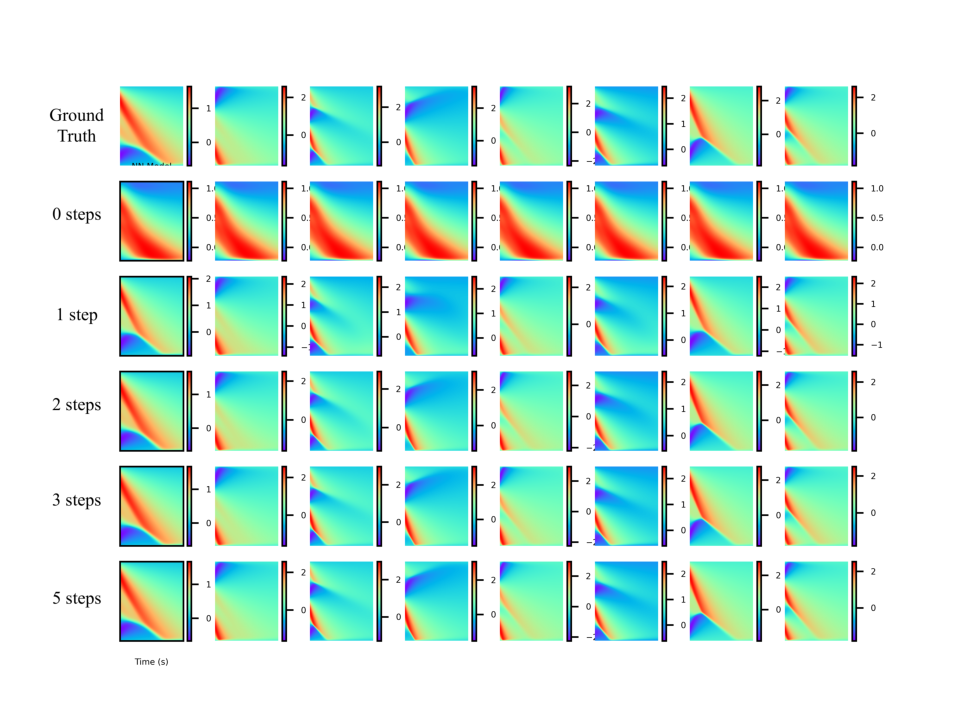
\includegraphics[width=0.7\linewidth]{figures/burgers_meta.pdf}
\caption{Solutions to Burgers's Equations with varying initial conditions, and boundary conditions. Top: ground truth finite element solution. Second row: solution represented by Meta-PDE initial neural network parameters. Third row onwards: solution after each gradient step in the Meta-PDE inner loop.}
\label{fig:burgers_per_step}
\end{SCfigure}

Figure \ref{fig:burgers_summary} shows the mean squared error (MSE) of each solution and solving time required for the desired accuracy. We see that Meta-PDE learns to output accurate solutions, and when run on the same CPU is about $500\times - 1,000\times$ faster than a finite element method with similar accuracy. 
%Unlike finite element models, Meta-PDE can be easily accelerated by a GPU, and on GPU we see close to $?\times$ speed up in deployment, leading to a $?\times$ speed increase over similar accuracy finite element models.


\begin{wrapfigure}[19]{r}{0.6\textwidth}
%\begin{figure}[htbp]
  \centering
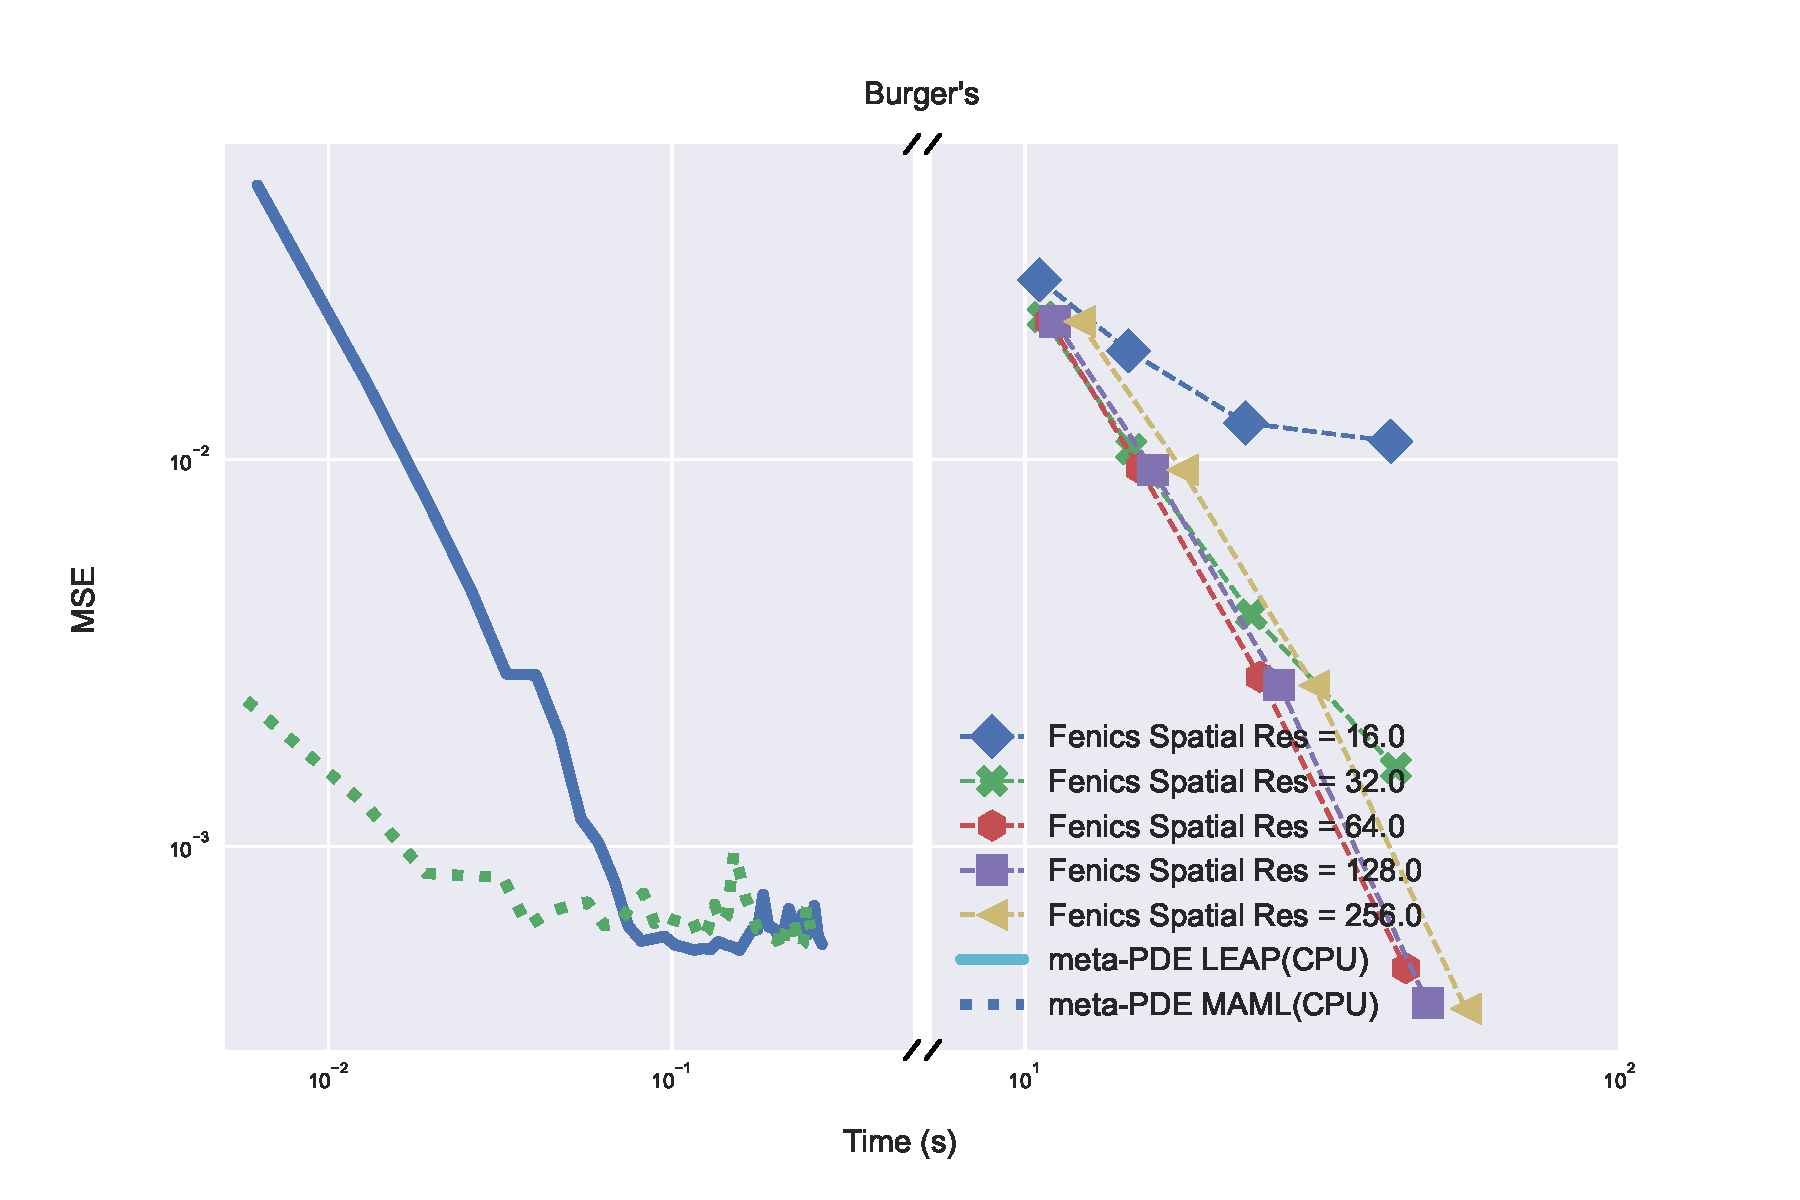
\includegraphics[width=1.0\linewidth]{figures/burgers.pdf}
\caption{MSE of each solution and the solving time required for the desired accuracy.}%
\label{fig:burgers_summary}%
\end{wrapfigure}


\subsection{Hyper-Elasticity Equation}
Hyper-elastic materials undergo large shape deformation when force is applied and the stress-strain relation for those materials are highly nonlinear. Rubber is a common example of hyper-elastic materials. the Hyper-Elasticity Equation models the deformation of those rubber-like materials under different external forces. In particular, we model a homogeneous and isotropic hyper-elasticity material under deformation when compressed uniaxially. We assume no additional body force (usually gravity) or additional traction force (usually dry friction against walls) applied to the structure. The goal is to model the final deformation displacement $u$, which maps the material position change from the initial reference position $\mathbf{X}$ to its current deformed location $\bm{x}$:
There are two different approaches to encode the loss function for the Hyper-Elasticity Equation. First, one could directly minimize the residual term in the original strong form, the same approach as we have done for the nonlinear Poisson's Equation and for the Burger's Equation. For example, \citet{abueidda2021meshless} has used the first approach to encode the loss function for PiNN. Alternatively, one can minimize the Helmholtz free energy of the system and find the corresponding minimizer $u$. We will use the second approach to solve the Hyper-Elasticity Equation. See Appendix \ref{appdx:hyperelasticity_pde} for details of the PDE formulation and loss function derivation.


We consider the deformation of a two-dimensional porous hyper-elastic material under compression. Their material properties could be very different from their solid counterparts. Because of these interesting differences, the hyper-elastic behavior of porous structures is an active field of research in material science \citep{overvelde2014relating, overvelde2012compaction}. Following the problem setup in \citep{overvelde2014relating}, we use the following parametrized equations to model the shape of the pores:
\begin{align*}
    x_1 &= r(\theta)\cos \theta, \, x_2 = r(\theta)\sin \theta \\
    r(\theta) &= r_0 \left[ 1 + c_1 \cos(4 \theta) + c_2\cos(8\theta)\right] \\
    r_0 &= \frac{L_0 \sqrt{2\phi_0}}{\sqrt{\pi \left(2 + x_1^2 + x_2^2\right)}}
\end{align*}
$\phi_0$ is the initial porosity of the structure, and it is sampled uniformly:  $\phi_0 \sim \mathcal{U}(0.0, 0.75)$ in our experiment setup. The parameter pair $(c_1, c_2)$ determines the shape of the pore, and we fixed them to $(0.0, 0.0)$ so that we only work with the circular porous shape. $L_0$ is the initial center-to-center distance between neighboring pores. We also fixed the distance $L_0$ so we work with fixed number of pores on the given material size. With the pore shape and the distance between pore centers $L_0$ fixed, the size of the pore determines the porosity of the structure. The porosity of the structure affects the macroscopic deformation behavior of the structure. 
%This setup is slighlt different from the ones done by \citep{overvelde2014relating}. They fixed porosity $\psi_0$ and the distance $L_0$, and studied how the shape of pores, i.e., $(c_1, c_2)$, affetcs the deformation behavior of the material. Figure \ref{fig:hyper-elasticity-example} shows three deformation example seen in experiments. 
%\begin{figure}[H]
%  \centering
%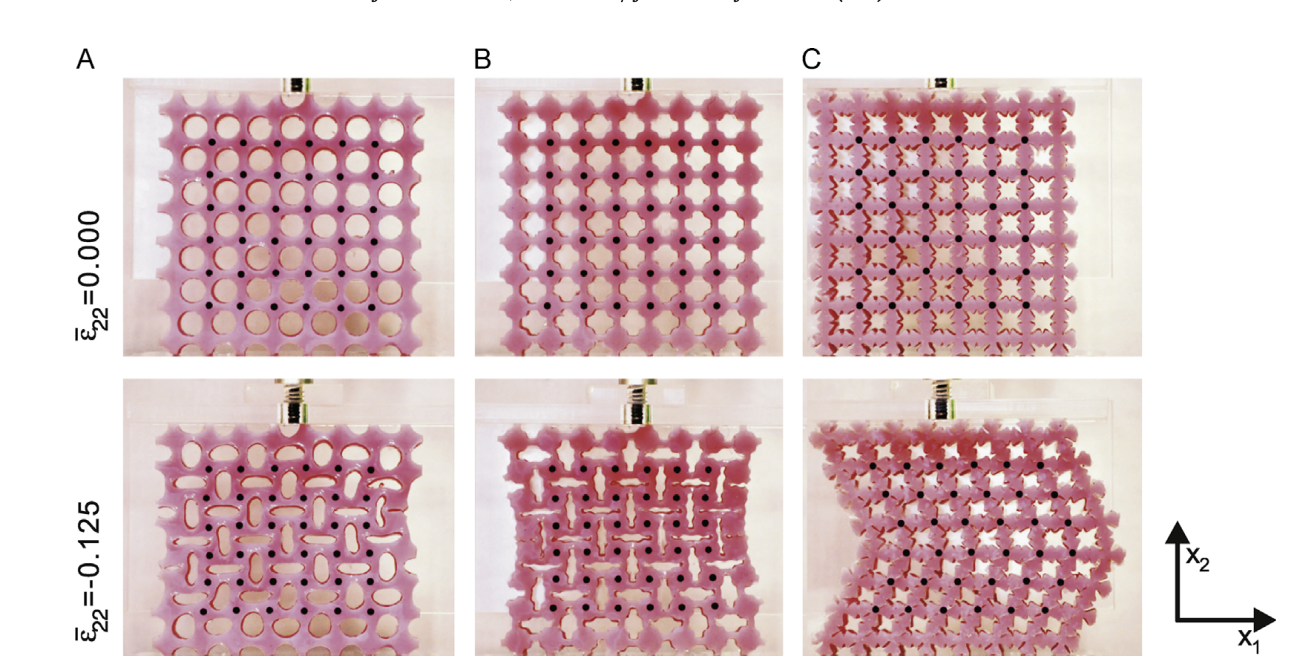
\includegraphics[width=0.8\linewidth]{figures/hyper_elasticity_example.png}
%\caption{Experimental images of three structures with pores shapes loaded under uniaxial compression. All structures are characterized by 50$\%$ porosity and the same strain is applied from above down. The shape of the pores affect the deformation behavior of the structure.
%Figure: \citet{overvelde2014relating}.}
%\label{fig:hyper-elasticity-example}%
%\end{figure}

The NN hyperparameter set is in Table \ref{tbl:hparams} and training hyperparameter details are in Table \ref{tbl:training}. Figure \ref{fig:hyperelasticity_per_step} shows the ground truth (baseline) solution for eight PDE problems used in the validation set. The same figure also shows the LEAP meta-learned initialization, which can quickly adapt to each PDE problems in 20 gradient steps. 

\begin{SCfigure}[1.0][htbp]
  \centering
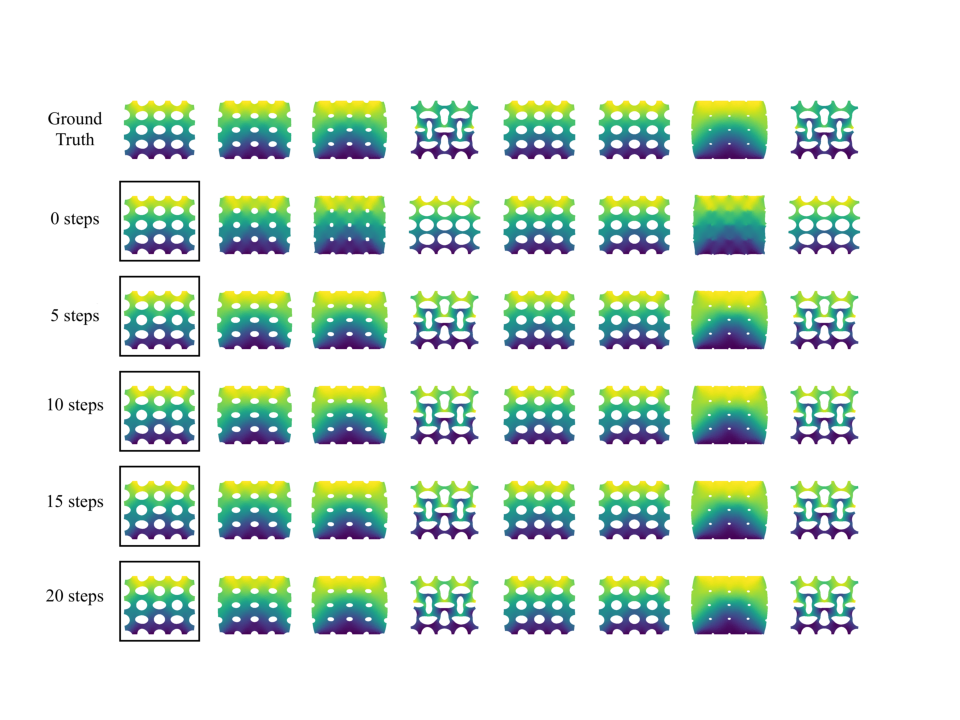
\includegraphics[width=0.6\linewidth]{figures/hyper_elasticity_circle_meta.pdf} 
\caption{Solutions to Hyper-Elasticity Equations with varying domains. Top: ground truth finite element solution. Second row: solution represented by Meta-PDE initial neural network parameters. Third row onwards: solution after each gradient step in the Meta-PDE inner loop.}
\label{fig:hyperelasticity_per_step}
\end{SCfigure}

Figure \ref{fig:hyperelasricity_summary} shows the mean squared error (MSE) of each solution and solving time required for the desired accuracy. We see that Meta-PDE learns to output accurate solutions, and when run on the same CPU is about $10\times - 100\times$ faster than a finite element method with similar accuracy.
%and about $?\times$ more accurate than a finite element method with the same computation cost. Unlike finite element models, Meta-PDE can be easily accelerated by a GPU, and on GPU we see close to $?\times$ speed up in deployment, leading to a $?\times$ speed increase over similar accuracy finite element models.

\section{Discussion}
\paragraph{Meta-PDE Methods Comparison} MAML-based Meta-PDE method outperforms LEAP-based Meta-PDE method during deployment time in both accuracy and speed. The superior performance is a results of smaller neural network architecture and fewer inner steps. The per-step and per-parameter step size serves as the main contributor to such good performance for MMAL. However, we observe that it takes longer to train the MAML-based meta-learning model because in MAML's meta-learning algorithm, we need to unroll each inner task during the training, and perform backpropagation through each inner-step through automatic differentiation. Such computation imposes a large memory constraint especially when we train the meta-learning model on a GPU with 16 GB memory. Alternatively, such computation takes a longer time when we use checkpointing to reduce the memory footprint. In two of our three experiments, we needed to use checkpoints so that we could fit the training on a single GPU. 

LEAP-based method, on the other hand, takes longer to adapt to new tasks due to the larger neural network sizes and more training steps. The advantage of LEAP-based Meta-PDE method lies in the meta-training process. The LEAP algorithm provides an analytical solution for the meta-gradient. The analytical solution circumvents the automatic differentiation computation needed in MAML. As a result, LEAP has a much smaller memory footprint compared to MAML. Such a computation advantage also comes at the cost of model flexibility. In particular, the MAML-based Meta-PDE method benefits from having a meta-learned per-state per-parameter step size. Having an analytical form for the meta-gradients implies that such a feature can not be easily incorporated into the LEAP algorithm. Furthermore, unlike MAML, LEAP requires the user to input the learning rate for the inner loop. Empirically, the model convergence is sensitive to the inner learning rate. As a result, the hyperparameter tuning for LEAP-based Meta-PDE method is more arduous compared to MAML. 

\paragraph{Task Domain Generalizability} In our study, we confine the meta-learner's task pool to one type of PDE, and for each type of PDE we define the task pool by having different parameterizations of the same PDE type. As we increase the task pool size, either by increasing the range of parameters or by increasing the number of paraemeters, the meta-learning tasks becomes harder. As a result, we need to use larger network architecture, increase the number of inner trainnig steps, increase meta-learner's training time to allow it to converge. The quality of the final model produced by the meta-PDE method also deteriorates. Namely, the accuracy of the solution to PDE problems after $K$ training step becomes worse. For example, in Figure \ref{fig:elasticity_flower_meta} we looked at a how different pore shapes affect the macroscopic behavior of the material. It is original problem studied by \citet{overvelde2014relating}. Neither LEAP-based Meta-PDE method nor MAML-based Meta-PDE method found a model that can solve particular instances of the PDE to a satisfactory accuracy. \\
\begin{figure}[h]
  \centering
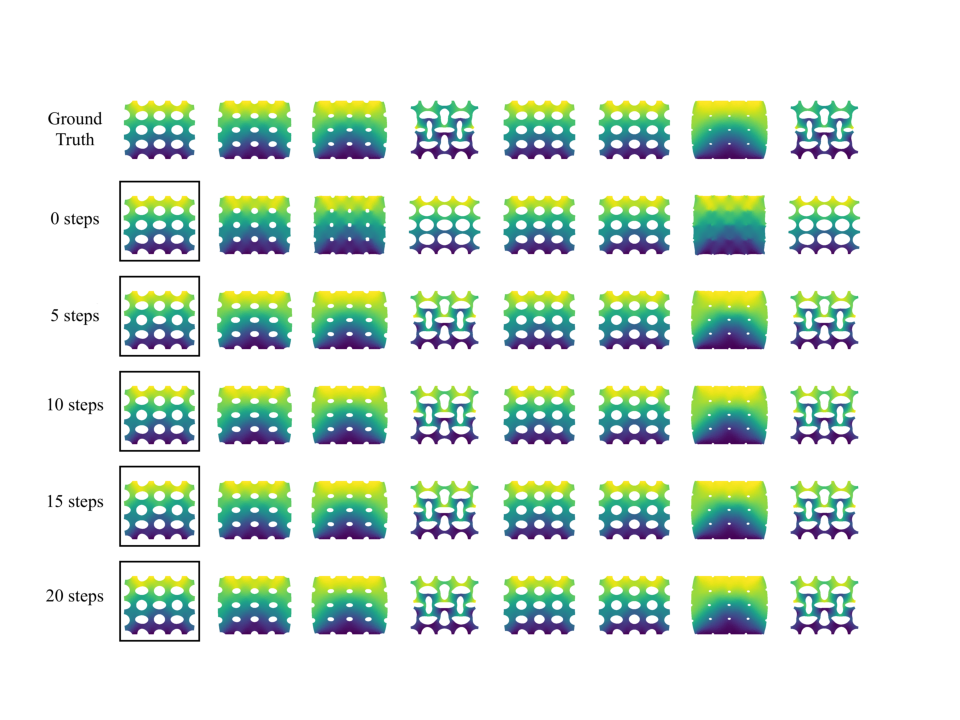
\includegraphics[width=0.8\linewidth]{figures/hyper_elasticity_circle_meta.pdf}
\caption{Solutions to hyper-elasticity equations with varying porous shape. Top: ground truth finite element solution. Second row: solution represented by Meta-PDE initial neural network parameters. Third row onwards: solution after each gradient step in the Meta-PDE inner loop. Looking at the bottom row, we can see that our meta-PDE based method fails to find a satisfactory solution. }%
\label{fig:elasticity_flower_meta}%
\end{figure}

\paragraph{Hard-to-solve PiNNs}  
In our study, we encountered examples of PDEs such that our Meta-PDE method cannot find meaningful solutions for task pool with a meaningful size (we exclude task pools that are trivial). These PDEs include ones that PiNNs find hard to solve - Navier-Stokes Equations, 2D Burger's Equations. One possible cause for such an issue is the simplicity in our neural network architecture. In all of our experiments, We only used vanilla FCNN as our main architecture choice. However, many works have been done to tailor NN architecture design to solve these problems under the PiNN setting. For example, the attention-like model is used to fit PDE solutions in \citet{wang2020understanding}). In future study, we are interested in seeing whether one could adopt more complex NN designs into the Meta-PDE method. We are hoping to see that a better architecture design for these hard-to-solve PDEs might improve Meta-PDE's performance.
\section{Conclusion}
We presented Meta-PDE, a surrogate model uses meta-learning to amortize PDE solving across classes of PDEs with complex and varying geometries and governing equations. Meta-PDE takes as input the governing equations themselves and a sampler for the PDE domain and boundary, thus remaining as close as possible in API to the fundamental representation of the PDE in terms of governing equations and domain. This avoids having to fix a parametric representation of geometry, governing equations and solution for the class of PDEs to be amortized. We show on three problems: nonlinear Poisson's Equation, Burger's Equation and Hyperelasiticty Equation that Meta-PDE can learn to output accurate solutions. In some cases, we observe a significantly more favorable accuracy/speed trade-off than a baseline finite element solver. The Meta-PDE method consists of two different implementations, differing in their meta-learning algorithms (MAML v.s. LEAP). Based on the three sets of experimentation, we observe that MAML-based Meta-PDE method yields superior speed/accuracy trade-off during deployment time. However, it comes as a cost of higher memory footprint during meta-training. The high-memory footprint imposes challanges when one want to use larger or more complex neural network architectures to solve complex PDE problems. The meta-training time for MAML-based Meta-PDE method is also slightly longer than its LEAP counterpart. The LEAP-based Meta-PDE method, on the other hand, has a worse speed/accuracy trade-off during deployment time but the meta-training time is slightly shorter. However, since the inner-loop learning rate is not meta-learnable for LEAP, the LEAP-based Meta-PDE training process is more sensitive to this hyperparameters. 

\bibliographystyle{plainnat}
\bibliography{references}
\end{document}
